% **************************************************************************************************************
% A Classic Thesis Style
% An Homage to The Elements of Typographic Style
%
% Copyright (C) 2012 Andr\'e Miede http://www.miede.de
%
% If you like the style then I would appreciate a postcard. My address 
% can be found in the file ClassicThesis.pdf. A collection of the 
% postcards I received so far is available online at 
% http://postcards.miede.de
%
% License:
% This program is free software; you can redistribute it and/or modify
% it under the terms of the GNU General Public License as published by
% the Free Software Foundation; either version 2 of the License, or
% (at your option) any later version.
%
% This program is distributed in the hope that it will be useful,
% but WITHOUT ANY WARRANTY; without even the implied warranty of
% MERCHANTABILITY or FITNESS FOR A PARTICULAR PURPOSE.  See the
% GNU General Public License for more details.
%
% You should have received a copy of the GNU General Public License
% along with this program; see the file COPYING.  If not, write to
% the Free Software Foundation, Inc., 59 Temple Place - Suite 330,
% Boston, MA 02111-1307, USA.
%
% **************************************************************************************************************
% Note:
%    * You must not use "u etc. in strings/commands that will be spaced out (use \"u or real umlauts instead)
%    * New enumeration (small caps): \begin{aenumerate} \end{aenumerate}
%    * For margin notes: \marginpar or \graffito{}
%    * Do not use bold fonts in this style, it is designed around them
%    * Use tables as in the examples
%    * See classicthesis-preamble.sty for useful commands
% **************************************************************************************************************
% To Do:
%		 * [high] Check this out: http://www.golatex.de/koma-script-warnung-in-verbindung-mit-listings-package-t2058.html
%    * [medium] mathbb in section-titles/chapter-titles => disappears somehow in headlines!!!
% **************************************************************************************************************
\documentclass[ twoside,openright,titlepage,numbers=noenddot,headinclude,%1headlines,% letterpaper a4paper
                footinclude=true,cleardoublepage=empty,abstractoff, % <--- obsolete, remove (todo)
                BCOR=5mm,paper=a4,fontsize=11pt,%11pt,a4paper,%
                ngerman,american,%
                ]{scrreprt}

%********************************************************************
% Note: Make all your adjustments in here
%*******************************************************
% ****************************************************************************************************
% classicthesis-config.tex 
% formerly known as loadpackages.sty, classicthesis-ldpkg.sty, and classicthesis-preamble.sty 
% Use it at the beginning of your ClassicThesis.tex, or as a LaTeX Preamble 
% in your ClassicThesis.{tex,lyx} with % ****************************************************************************************************
% classicthesis-config.tex 
% formerly known as loadpackages.sty, classicthesis-ldpkg.sty, and classicthesis-preamble.sty 
% Use it at the beginning of your ClassicThesis.tex, or as a LaTeX Preamble 
% in your ClassicThesis.{tex,lyx} with % ****************************************************************************************************
% classicthesis-config.tex 
% formerly known as loadpackages.sty, classicthesis-ldpkg.sty, and classicthesis-preamble.sty 
% Use it at the beginning of your ClassicThesis.tex, or as a LaTeX Preamble 
% in your ClassicThesis.{tex,lyx} with \input{classicthesis-config}
% ****************************************************************************************************  
% If you like the classicthesis, then I would appreciate a postcard. 
% My address can be found in the file ClassicThesis.pdf. A collection 
% of the postcards I received so far is available online at 
% http://postcards.miede.de
% ****************************************************************************************************

% ****************************************************************************************************
% 1. Configure classicthesis for your needs here, e.g., remove "drafting" below 
% in order to deactivate the time-stamp on the pages
% ****************************************************************************************************
\PassOptionsToPackage{eulerchapternumbers,listings,drafting,%
				 pdfspacing,%floatperchapter,%linedheaders,%
				 subfig,beramono,eulermath,parts}{classicthesis}										
% ********************************************************************
% Available options for classicthesis.sty 
% (see ClassicThesis.pdf for more information):
% drafting
% parts nochapters linedheaders
% eulerchapternumbers beramono eulermath pdfspacing minionprospacing
% tocaligned dottedtoc manychapters
% listings floatperchapter subfig
% ********************************************************************

% ********************************************************************
% Triggers for this config
% ******************************************************************** 
\usepackage{ifthen}
\newboolean{enable-backrefs} % enable backrefs in the bibliography
\setboolean{enable-backrefs}{false} % true false
% ****************************************************************************************************


% ****************************************************************************************************
% 2. Personal data and user ad-hoc commands
% ****************************************************************************************************
\newcommand{\myTitle}{Design and Implementation of Cloud Connected Mobile Applications\xspace}
\newcommand{\mySubtitle}{Building a Job Portal Aggregator for the MHM eRecruiting Systems\xspace}
\newcommand{\myDegree}{Bachelor of Science (B.Sc.)\xspace}
\newcommand{\myName}{Patricio Javier Cano Chavez\xspace}\newcommand{\myProf}{Put name here\xspace}
\newcommand{\myOtherProf}{Put name here\xspace}
\newcommand{\mySupervisor}{Put name here\xspace}
\newcommand{\myFaculty}{Put data here\xspace}
\newcommand{\myDepartment}{Put data here\xspace}
\newcommand{\myUni}{Put data here\xspace}
\newcommand{\myLocation}{Stuttgart\xspace}
\newcommand{\myTime}{October 2013\xspace}
\newcommand{\myVersion}{version 0.5\xspace}

% ********************************************************************
% Setup, finetuning, and useful commands
% ********************************************************************
\newcounter{dummy} % necessary for correct hyperlinks (to index, bib, etc.)
\newlength{\abcd} % for ab..z string length calculation
\providecommand{\mLyX}{L\kern-.1667em\lower.25em\hbox{Y}\kern-.125emX\@}
\newcommand{\ie}{i.\,e.}
\newcommand{\Ie}{I.\,e.}
\newcommand{\eg}{e.\,g.}
\newcommand{\Eg}{E.\,g.} 
% ****************************************************************************************************


% ****************************************************************************************************
% 3. Loading some handy packages
% ****************************************************************************************************
% ******************************************************************** 
% Packages with options that might require adjustments
% ******************************************************************** 
\PassOptionsToPackage{latin9}{inputenc}	% latin9 (ISO-8859-9) = latin1+"Euro sign"
 \usepackage{inputenc}				

%\PassOptionsToPackage{ngerman,american}{babel}   % change this to your language(s)
% Spanish languages need extra options in order to work with this template
%\PassOptionsToPackage{spanish,es-lcroman}{babel}
 \usepackage{babel}					

\PassOptionsToPackage{square,numbers}{natbib}
 \usepackage{natbib}	
 %\usepackage{bibtex}				

\PassOptionsToPackage{fleqn}{amsmath}		% math environments and more by the AMS 
 \usepackage{amsmath}

% ******************************************************************** 
% General useful packages
% ******************************************************************** 
\PassOptionsToPackage{T1}{fontenc} % T2A for cyrillics
	\usepackage{fontenc}     
\usepackage{textcomp} % fix warning with missing font shapes
\usepackage{scrhack} % fix warnings when using KOMA with listings package          
\usepackage{xspace} % to get the spacing after macros right  
\usepackage{mparhack} % get marginpar right
\usepackage{fixltx2e} % fixes some LaTeX stuff 
\PassOptionsToPackage{printonlyused,smaller}{acronym}
	\usepackage{acronym} % nice macros for handling all acronyms in the thesis
%\renewcommand*{\acsfont}[1]{\textssc{#1}} % for MinionPro
\renewcommand{\bflabel}[1]{{#1}\hfill} % fix the list of acronyms
% ****************************************************************************************************


% ****************************************************************************************************
% 4. Setup floats: tables, (sub)figures, and captions
% ****************************************************************************************************
\usepackage{tabularx} % better tables
	\setlength{\extrarowheight}{3pt} % increase table row height
\newcommand{\tableheadline}[1]{\multicolumn{1}{c}{\spacedlowsmallcaps{#1}}}
\newcommand{\myfloatalign}{\centering} % to be used with each float for alignment
\usepackage{caption}
\captionsetup{format=hang,font=small}
\usepackage{subfig}
\usepackage{float}
\restylefloat{figure}
\usepackage{parskip}
%**my packages**
\usepackage[super]{nth}
\usepackage[hyphens]{url}
\usepackage{pifont} 
% ****************************************************************************************************


% ****************************************************************************************************
% 5. Setup code listings
% ****************************************************************************************************
\usepackage{listings} 
%\lstset{emph={trueIndex,root},emphstyle=\color{BlueViolet}}%\underbar} % for special keywords
\lstset{language=[LaTeX]Tex,%C++,
    keywordstyle=\color{RoyalBlue},%\bfseries,
    basicstyle=\small\ttfamily,
    %identifierstyle=\color{NavyBlue},
    commentstyle=\color{Green}\ttfamily,
    stringstyle=\rmfamily,
    numbers=none,%left,%
    numberstyle=\scriptsize,%\tiny
    stepnumber=5,
    numbersep=8pt,
    showstringspaces=false,
    breaklines=true,
    frameround=ftff,
    frame=single,
    belowcaptionskip=.75\baselineskip
    %frame=L
} 
% ****************************************************************************************************    		   


% ****************************************************************************************************
% 6. PDFLaTeX, hyperreferences and citation backreferences
% ****************************************************************************************************
% ********************************************************************
% Using PDFLaTeX
% ********************************************************************
\PassOptionsToPackage{pdftex,hyperfootnotes=false,pdfpagelabels}{hyperref}
	\usepackage{hyperref}  % backref linktocpage pagebackref
\pdfcompresslevel=9
\pdfadjustspacing=1 
\PassOptionsToPackage{pdftex}{graphicx}
	\usepackage{graphicx} 

% ********************************************************************
% Setup the style of the backrefs from the bibliography
% (translate the options to any language you use)
% ********************************************************************
\newcommand{\backrefnotcitedstring}{\relax}%(Not cited.)
\newcommand{\backrefcitedsinglestring}[1]{(Cited on page~#1.)}
\newcommand{\backrefcitedmultistring}[1]{(Cited on pages~#1.)}
\ifthenelse{\boolean{enable-backrefs}}%
{%
		\PassOptionsToPackage{hyperpageref}{backref}
		\usepackage{backref} % to be loaded after hyperref package 
		   \renewcommand{\backreftwosep}{ and~} % separate 2 pages
		   \renewcommand{\backreflastsep}{, and~} % separate last of longer list
		   \renewcommand*{\backref}[1]{}  % disable standard
		   \renewcommand*{\backrefalt}[4]{% detailed backref
		      \ifcase #1 %
		         \backrefnotcitedstring%
		      \or%
		         \backrefcitedsinglestring{#2}%
		      \else%
		         \backrefcitedmultistring{#2}%
		      \fi}%
}{\relax}    

% ********************************************************************
% Hyperreferences
% ********************************************************************
\hypersetup{%
    %draft,	% = no hyperlinking at all (useful in b/w printouts)
    colorlinks=true, linktocpage=true, pdfstartpage=3, pdfstartview=FitV,%
    % uncomment the following line if you want to have black links (e.g., for printing)
    %colorlinks=false, linktocpage=false, pdfborder={0 0 0}, pdfstartpage=3, pdfstartview=FitV,% 
    breaklinks=true, pdfpagemode=UseNone, pageanchor=true, pdfpagemode=UseOutlines,%
    plainpages=false, bookmarksnumbered, bookmarksopen=true, bookmarksopenlevel=1,%
    hypertexnames=true, pdfhighlight=/O,%nesting=true,%frenchlinks,%
    urlcolor=webbrown, linkcolor=RoyalBlue, citecolor=webgreen, %pagecolor=RoyalBlue,%
    %urlcolor=Black, linkcolor=Black, citecolor=Black, %pagecolor=Black,%
    pdftitle={\myTitle},%
    pdfauthor={\textcopyright\ \myName, \myUni, \myFaculty},%
    pdfsubject={},%
    pdfkeywords={},%
    pdfcreator={pdfLaTeX},%
    pdfproducer={LaTeX with hyperref and classicthesis}%
}   

% ********************************************************************
% Setup autoreferences
% ********************************************************************
% There are some issues regarding autorefnames
% http://www.ureader.de/msg/136221647.aspx
% http://www.tex.ac.uk/cgi-bin/texfaq2html?label=latexwords
% you have to redefine the makros for the 
% language you use, e.g., american, ngerman
% (as chosen when loading babel/AtBeginDocument)
% ********************************************************************
\makeatletter
\@ifpackageloaded{babel}%
    {%
       \addto\extrasamerican{%
					\renewcommand*{\figureautorefname}{Figure}%
					\renewcommand*{\tableautorefname}{Table}%
					\renewcommand*{\partautorefname}{Part}%
					\renewcommand*{\chapterautorefname}{Chapter}%
					\renewcommand*{\sectionautorefname}{Section}%
					\renewcommand*{\subsectionautorefname}{Section}%
					\renewcommand*{\subsubsectionautorefname}{Section}% 	
				}%
       \addto\extrasngerman{% 
					\renewcommand*{\paragraphautorefname}{Absatz}%
					\renewcommand*{\subparagraphautorefname}{Unterabsatz}%
					\renewcommand*{\footnoteautorefname}{Fu\"snote}%
					\renewcommand*{\FancyVerbLineautorefname}{Zeile}%
					\renewcommand*{\theoremautorefname}{Theorem}%
					\renewcommand*{\appendixautorefname}{Anhang}%
					\renewcommand*{\equationautorefname}{Gleichung}%        
					\renewcommand*{\itemautorefname}{Punkt}%
				}%	
			% Fix to getting autorefs for subfigures right (thanks to Belinda Vogt for changing the definition)
			\providecommand{\subfigureautorefname}{\figureautorefname}%  			
    }{\relax}
\makeatother


% ****************************************************************************************************
% 7. Last calls before the bar closes
% ****************************************************************************************************
% ********************************************************************
% Development Stuff
% ********************************************************************
\listfiles
%\PassOptionsToPackage{l2tabu,orthodox,abort}{nag}
%	\usepackage{nag}
%\PassOptionsToPackage{warning, all}{onlyamsmath}
%	\usepackage{onlyamsmath}

% ********************************************************************
% Last, but not least...
% ********************************************************************
\usepackage{classicthesis} 
% ****************************************************************************************************


% ****************************************************************************************************
% 8. Further adjustments (experimental)
% ****************************************************************************************************
% ********************************************************************
% Changing the text area
% ********************************************************************
%\linespread{1.05} % a bit more for Palatino
%\areaset[current]{312pt}{761pt} % 686 (factor 2.2) + 33 head + 42 head \the\footskip
%\setlength{\marginparwidth}{7em}%
%\setlength{\marginparsep}{2em}%

% ********************************************************************
% Using different fonts
% ********************************************************************
%\usepackage[oldstylenums]{kpfonts} % oldstyle notextcomp
%\usepackage[osf]{libertine}
%\usepackage{hfoldsty} % Computer Modern with osf
%\usepackage[light,condensed,math]{iwona}
%\renewcommand{\sfdefault}{iwona}
%\usepackage{lmodern} % <-- no osf support :-(
%\usepackage[urw-garamond]{mathdesign} <-- no osf support :-(
% ****************************************************************************************************

% ****************************************************************************************************  
% If you like the classicthesis, then I would appreciate a postcard. 
% My address can be found in the file ClassicThesis.pdf. A collection 
% of the postcards I received so far is available online at 
% http://postcards.miede.de
% ****************************************************************************************************

% ****************************************************************************************************
% 1. Configure classicthesis for your needs here, e.g., remove "drafting" below 
% in order to deactivate the time-stamp on the pages
% ****************************************************************************************************
\PassOptionsToPackage{eulerchapternumbers,listings,drafting,%
				 pdfspacing,%floatperchapter,%linedheaders,%
				 subfig,beramono,eulermath,parts}{classicthesis}										
% ********************************************************************
% Available options for classicthesis.sty 
% (see ClassicThesis.pdf for more information):
% drafting
% parts nochapters linedheaders
% eulerchapternumbers beramono eulermath pdfspacing minionprospacing
% tocaligned dottedtoc manychapters
% listings floatperchapter subfig
% ********************************************************************

% ********************************************************************
% Triggers for this config
% ******************************************************************** 
\usepackage{ifthen}
\newboolean{enable-backrefs} % enable backrefs in the bibliography
\setboolean{enable-backrefs}{false} % true false
% ****************************************************************************************************


% ****************************************************************************************************
% 2. Personal data and user ad-hoc commands
% ****************************************************************************************************
\newcommand{\myTitle}{Design and Implementation of Cloud Connected Mobile Applications\xspace}
\newcommand{\mySubtitle}{Building a Job Portal Aggregator for the MHM eRecruiting Systems\xspace}
\newcommand{\myDegree}{Bachelor of Science (B.Sc.)\xspace}
\newcommand{\myName}{Patricio Javier Cano Chavez\xspace}\newcommand{\myProf}{Put name here\xspace}
\newcommand{\myOtherProf}{Put name here\xspace}
\newcommand{\mySupervisor}{Put name here\xspace}
\newcommand{\myFaculty}{Put data here\xspace}
\newcommand{\myDepartment}{Put data here\xspace}
\newcommand{\myUni}{Put data here\xspace}
\newcommand{\myLocation}{Stuttgart\xspace}
\newcommand{\myTime}{October 2013\xspace}
\newcommand{\myVersion}{version 0.5\xspace}

% ********************************************************************
% Setup, finetuning, and useful commands
% ********************************************************************
\newcounter{dummy} % necessary for correct hyperlinks (to index, bib, etc.)
\newlength{\abcd} % for ab..z string length calculation
\providecommand{\mLyX}{L\kern-.1667em\lower.25em\hbox{Y}\kern-.125emX\@}
\newcommand{\ie}{i.\,e.}
\newcommand{\Ie}{I.\,e.}
\newcommand{\eg}{e.\,g.}
\newcommand{\Eg}{E.\,g.} 
% ****************************************************************************************************


% ****************************************************************************************************
% 3. Loading some handy packages
% ****************************************************************************************************
% ******************************************************************** 
% Packages with options that might require adjustments
% ******************************************************************** 
\PassOptionsToPackage{latin9}{inputenc}	% latin9 (ISO-8859-9) = latin1+"Euro sign"
 \usepackage{inputenc}				

%\PassOptionsToPackage{ngerman,american}{babel}   % change this to your language(s)
% Spanish languages need extra options in order to work with this template
%\PassOptionsToPackage{spanish,es-lcroman}{babel}
 \usepackage{babel}					

\PassOptionsToPackage{square,numbers}{natbib}
 \usepackage{natbib}	
 %\usepackage{bibtex}				

\PassOptionsToPackage{fleqn}{amsmath}		% math environments and more by the AMS 
 \usepackage{amsmath}

% ******************************************************************** 
% General useful packages
% ******************************************************************** 
\PassOptionsToPackage{T1}{fontenc} % T2A for cyrillics
	\usepackage{fontenc}     
\usepackage{textcomp} % fix warning with missing font shapes
\usepackage{scrhack} % fix warnings when using KOMA with listings package          
\usepackage{xspace} % to get the spacing after macros right  
\usepackage{mparhack} % get marginpar right
\usepackage{fixltx2e} % fixes some LaTeX stuff 
\PassOptionsToPackage{printonlyused,smaller}{acronym}
	\usepackage{acronym} % nice macros for handling all acronyms in the thesis
%\renewcommand*{\acsfont}[1]{\textssc{#1}} % for MinionPro
\renewcommand{\bflabel}[1]{{#1}\hfill} % fix the list of acronyms
% ****************************************************************************************************


% ****************************************************************************************************
% 4. Setup floats: tables, (sub)figures, and captions
% ****************************************************************************************************
\usepackage{tabularx} % better tables
	\setlength{\extrarowheight}{3pt} % increase table row height
\newcommand{\tableheadline}[1]{\multicolumn{1}{c}{\spacedlowsmallcaps{#1}}}
\newcommand{\myfloatalign}{\centering} % to be used with each float for alignment
\usepackage{caption}
\captionsetup{format=hang,font=small}
\usepackage{subfig}
\usepackage{float}
\restylefloat{figure}
\usepackage{parskip}
%**my packages**
\usepackage[super]{nth}
\usepackage[hyphens]{url}
\usepackage{pifont} 
% ****************************************************************************************************


% ****************************************************************************************************
% 5. Setup code listings
% ****************************************************************************************************
\usepackage{listings} 
%\lstset{emph={trueIndex,root},emphstyle=\color{BlueViolet}}%\underbar} % for special keywords
\lstset{language=[LaTeX]Tex,%C++,
    keywordstyle=\color{RoyalBlue},%\bfseries,
    basicstyle=\small\ttfamily,
    %identifierstyle=\color{NavyBlue},
    commentstyle=\color{Green}\ttfamily,
    stringstyle=\rmfamily,
    numbers=none,%left,%
    numberstyle=\scriptsize,%\tiny
    stepnumber=5,
    numbersep=8pt,
    showstringspaces=false,
    breaklines=true,
    frameround=ftff,
    frame=single,
    belowcaptionskip=.75\baselineskip
    %frame=L
} 
% ****************************************************************************************************    		   


% ****************************************************************************************************
% 6. PDFLaTeX, hyperreferences and citation backreferences
% ****************************************************************************************************
% ********************************************************************
% Using PDFLaTeX
% ********************************************************************
\PassOptionsToPackage{pdftex,hyperfootnotes=false,pdfpagelabels}{hyperref}
	\usepackage{hyperref}  % backref linktocpage pagebackref
\pdfcompresslevel=9
\pdfadjustspacing=1 
\PassOptionsToPackage{pdftex}{graphicx}
	\usepackage{graphicx} 

% ********************************************************************
% Setup the style of the backrefs from the bibliography
% (translate the options to any language you use)
% ********************************************************************
\newcommand{\backrefnotcitedstring}{\relax}%(Not cited.)
\newcommand{\backrefcitedsinglestring}[1]{(Cited on page~#1.)}
\newcommand{\backrefcitedmultistring}[1]{(Cited on pages~#1.)}
\ifthenelse{\boolean{enable-backrefs}}%
{%
		\PassOptionsToPackage{hyperpageref}{backref}
		\usepackage{backref} % to be loaded after hyperref package 
		   \renewcommand{\backreftwosep}{ and~} % separate 2 pages
		   \renewcommand{\backreflastsep}{, and~} % separate last of longer list
		   \renewcommand*{\backref}[1]{}  % disable standard
		   \renewcommand*{\backrefalt}[4]{% detailed backref
		      \ifcase #1 %
		         \backrefnotcitedstring%
		      \or%
		         \backrefcitedsinglestring{#2}%
		      \else%
		         \backrefcitedmultistring{#2}%
		      \fi}%
}{\relax}    

% ********************************************************************
% Hyperreferences
% ********************************************************************
\hypersetup{%
    %draft,	% = no hyperlinking at all (useful in b/w printouts)
    colorlinks=true, linktocpage=true, pdfstartpage=3, pdfstartview=FitV,%
    % uncomment the following line if you want to have black links (e.g., for printing)
    %colorlinks=false, linktocpage=false, pdfborder={0 0 0}, pdfstartpage=3, pdfstartview=FitV,% 
    breaklinks=true, pdfpagemode=UseNone, pageanchor=true, pdfpagemode=UseOutlines,%
    plainpages=false, bookmarksnumbered, bookmarksopen=true, bookmarksopenlevel=1,%
    hypertexnames=true, pdfhighlight=/O,%nesting=true,%frenchlinks,%
    urlcolor=webbrown, linkcolor=RoyalBlue, citecolor=webgreen, %pagecolor=RoyalBlue,%
    %urlcolor=Black, linkcolor=Black, citecolor=Black, %pagecolor=Black,%
    pdftitle={\myTitle},%
    pdfauthor={\textcopyright\ \myName, \myUni, \myFaculty},%
    pdfsubject={},%
    pdfkeywords={},%
    pdfcreator={pdfLaTeX},%
    pdfproducer={LaTeX with hyperref and classicthesis}%
}   

% ********************************************************************
% Setup autoreferences
% ********************************************************************
% There are some issues regarding autorefnames
% http://www.ureader.de/msg/136221647.aspx
% http://www.tex.ac.uk/cgi-bin/texfaq2html?label=latexwords
% you have to redefine the makros for the 
% language you use, e.g., american, ngerman
% (as chosen when loading babel/AtBeginDocument)
% ********************************************************************
\makeatletter
\@ifpackageloaded{babel}%
    {%
       \addto\extrasamerican{%
					\renewcommand*{\figureautorefname}{Figure}%
					\renewcommand*{\tableautorefname}{Table}%
					\renewcommand*{\partautorefname}{Part}%
					\renewcommand*{\chapterautorefname}{Chapter}%
					\renewcommand*{\sectionautorefname}{Section}%
					\renewcommand*{\subsectionautorefname}{Section}%
					\renewcommand*{\subsubsectionautorefname}{Section}% 	
				}%
       \addto\extrasngerman{% 
					\renewcommand*{\paragraphautorefname}{Absatz}%
					\renewcommand*{\subparagraphautorefname}{Unterabsatz}%
					\renewcommand*{\footnoteautorefname}{Fu\"snote}%
					\renewcommand*{\FancyVerbLineautorefname}{Zeile}%
					\renewcommand*{\theoremautorefname}{Theorem}%
					\renewcommand*{\appendixautorefname}{Anhang}%
					\renewcommand*{\equationautorefname}{Gleichung}%        
					\renewcommand*{\itemautorefname}{Punkt}%
				}%	
			% Fix to getting autorefs for subfigures right (thanks to Belinda Vogt for changing the definition)
			\providecommand{\subfigureautorefname}{\figureautorefname}%  			
    }{\relax}
\makeatother


% ****************************************************************************************************
% 7. Last calls before the bar closes
% ****************************************************************************************************
% ********************************************************************
% Development Stuff
% ********************************************************************
\listfiles
%\PassOptionsToPackage{l2tabu,orthodox,abort}{nag}
%	\usepackage{nag}
%\PassOptionsToPackage{warning, all}{onlyamsmath}
%	\usepackage{onlyamsmath}

% ********************************************************************
% Last, but not least...
% ********************************************************************
\usepackage{classicthesis} 
% ****************************************************************************************************


% ****************************************************************************************************
% 8. Further adjustments (experimental)
% ****************************************************************************************************
% ********************************************************************
% Changing the text area
% ********************************************************************
%\linespread{1.05} % a bit more for Palatino
%\areaset[current]{312pt}{761pt} % 686 (factor 2.2) + 33 head + 42 head \the\footskip
%\setlength{\marginparwidth}{7em}%
%\setlength{\marginparsep}{2em}%

% ********************************************************************
% Using different fonts
% ********************************************************************
%\usepackage[oldstylenums]{kpfonts} % oldstyle notextcomp
%\usepackage[osf]{libertine}
%\usepackage{hfoldsty} % Computer Modern with osf
%\usepackage[light,condensed,math]{iwona}
%\renewcommand{\sfdefault}{iwona}
%\usepackage{lmodern} % <-- no osf support :-(
%\usepackage[urw-garamond]{mathdesign} <-- no osf support :-(
% ****************************************************************************************************

% ****************************************************************************************************  
% If you like the classicthesis, then I would appreciate a postcard. 
% My address can be found in the file ClassicThesis.pdf. A collection 
% of the postcards I received so far is available online at 
% http://postcards.miede.de
% ****************************************************************************************************

% ****************************************************************************************************
% 1. Configure classicthesis for your needs here, e.g., remove "drafting" below 
% in order to deactivate the time-stamp on the pages
% ****************************************************************************************************
\PassOptionsToPackage{eulerchapternumbers,listings,drafting,%
				 pdfspacing,%floatperchapter,%linedheaders,%
				 subfig,beramono,eulermath,parts}{classicthesis}										
% ********************************************************************
% Available options for classicthesis.sty 
% (see ClassicThesis.pdf for more information):
% drafting
% parts nochapters linedheaders
% eulerchapternumbers beramono eulermath pdfspacing minionprospacing
% tocaligned dottedtoc manychapters
% listings floatperchapter subfig
% ********************************************************************

% ********************************************************************
% Triggers for this config
% ******************************************************************** 
\usepackage{ifthen}
\newboolean{enable-backrefs} % enable backrefs in the bibliography
\setboolean{enable-backrefs}{false} % true false
% ****************************************************************************************************


% ****************************************************************************************************
% 2. Personal data and user ad-hoc commands
% ****************************************************************************************************
\newcommand{\myTitle}{Design and Implementation of Cloud Connected Mobile Applications\xspace}
\newcommand{\mySubtitle}{Building a Job Portal Aggregator for the MHM eRecruiting Systems\xspace}
\newcommand{\myDegree}{Bachelor of Science (B.Sc.)\xspace}
\newcommand{\myName}{Patricio Javier Cano Chavez\xspace}\newcommand{\myProf}{Put name here\xspace}
\newcommand{\myOtherProf}{Put name here\xspace}
\newcommand{\mySupervisor}{Put name here\xspace}
\newcommand{\myFaculty}{Put data here\xspace}
\newcommand{\myDepartment}{Put data here\xspace}
\newcommand{\myUni}{Put data here\xspace}
\newcommand{\myLocation}{Stuttgart\xspace}
\newcommand{\myTime}{October 2013\xspace}
\newcommand{\myVersion}{version 0.5\xspace}

% ********************************************************************
% Setup, finetuning, and useful commands
% ********************************************************************
\newcounter{dummy} % necessary for correct hyperlinks (to index, bib, etc.)
\newlength{\abcd} % for ab..z string length calculation
\providecommand{\mLyX}{L\kern-.1667em\lower.25em\hbox{Y}\kern-.125emX\@}
\newcommand{\ie}{i.\,e.}
\newcommand{\Ie}{I.\,e.}
\newcommand{\eg}{e.\,g.}
\newcommand{\Eg}{E.\,g.} 
% ****************************************************************************************************


% ****************************************************************************************************
% 3. Loading some handy packages
% ****************************************************************************************************
% ******************************************************************** 
% Packages with options that might require adjustments
% ******************************************************************** 
\PassOptionsToPackage{latin9}{inputenc}	% latin9 (ISO-8859-9) = latin1+"Euro sign"
 \usepackage{inputenc}				

%\PassOptionsToPackage{ngerman,american}{babel}   % change this to your language(s)
% Spanish languages need extra options in order to work with this template
%\PassOptionsToPackage{spanish,es-lcroman}{babel}
 \usepackage{babel}					

\PassOptionsToPackage{square,numbers}{natbib}
 \usepackage{natbib}	
 %\usepackage{bibtex}				

\PassOptionsToPackage{fleqn}{amsmath}		% math environments and more by the AMS 
 \usepackage{amsmath}

% ******************************************************************** 
% General useful packages
% ******************************************************************** 
\PassOptionsToPackage{T1}{fontenc} % T2A for cyrillics
	\usepackage{fontenc}     
\usepackage{textcomp} % fix warning with missing font shapes
\usepackage{scrhack} % fix warnings when using KOMA with listings package          
\usepackage{xspace} % to get the spacing after macros right  
\usepackage{mparhack} % get marginpar right
\usepackage{fixltx2e} % fixes some LaTeX stuff 
\PassOptionsToPackage{printonlyused,smaller}{acronym}
	\usepackage{acronym} % nice macros for handling all acronyms in the thesis
%\renewcommand*{\acsfont}[1]{\textssc{#1}} % for MinionPro
\renewcommand{\bflabel}[1]{{#1}\hfill} % fix the list of acronyms
% ****************************************************************************************************


% ****************************************************************************************************
% 4. Setup floats: tables, (sub)figures, and captions
% ****************************************************************************************************
\usepackage{tabularx} % better tables
	\setlength{\extrarowheight}{3pt} % increase table row height
\newcommand{\tableheadline}[1]{\multicolumn{1}{c}{\spacedlowsmallcaps{#1}}}
\newcommand{\myfloatalign}{\centering} % to be used with each float for alignment
\usepackage{caption}
\captionsetup{format=hang,font=small}
\usepackage{subfig}
\usepackage{float}
\restylefloat{figure}
\usepackage{parskip}
%**my packages**
\usepackage[super]{nth}
\usepackage[hyphens]{url}
\usepackage{pifont} 
% ****************************************************************************************************


% ****************************************************************************************************
% 5. Setup code listings
% ****************************************************************************************************
\usepackage{listings} 
%\lstset{emph={trueIndex,root},emphstyle=\color{BlueViolet}}%\underbar} % for special keywords
\lstset{language=[LaTeX]Tex,%C++,
    keywordstyle=\color{RoyalBlue},%\bfseries,
    basicstyle=\small\ttfamily,
    %identifierstyle=\color{NavyBlue},
    commentstyle=\color{Green}\ttfamily,
    stringstyle=\rmfamily,
    numbers=none,%left,%
    numberstyle=\scriptsize,%\tiny
    stepnumber=5,
    numbersep=8pt,
    showstringspaces=false,
    breaklines=true,
    frameround=ftff,
    frame=single,
    belowcaptionskip=.75\baselineskip
    %frame=L
} 
% ****************************************************************************************************    		   


% ****************************************************************************************************
% 6. PDFLaTeX, hyperreferences and citation backreferences
% ****************************************************************************************************
% ********************************************************************
% Using PDFLaTeX
% ********************************************************************
\PassOptionsToPackage{pdftex,hyperfootnotes=false,pdfpagelabels}{hyperref}
	\usepackage{hyperref}  % backref linktocpage pagebackref
\pdfcompresslevel=9
\pdfadjustspacing=1 
\PassOptionsToPackage{pdftex}{graphicx}
	\usepackage{graphicx} 

% ********************************************************************
% Setup the style of the backrefs from the bibliography
% (translate the options to any language you use)
% ********************************************************************
\newcommand{\backrefnotcitedstring}{\relax}%(Not cited.)
\newcommand{\backrefcitedsinglestring}[1]{(Cited on page~#1.)}
\newcommand{\backrefcitedmultistring}[1]{(Cited on pages~#1.)}
\ifthenelse{\boolean{enable-backrefs}}%
{%
		\PassOptionsToPackage{hyperpageref}{backref}
		\usepackage{backref} % to be loaded after hyperref package 
		   \renewcommand{\backreftwosep}{ and~} % separate 2 pages
		   \renewcommand{\backreflastsep}{, and~} % separate last of longer list
		   \renewcommand*{\backref}[1]{}  % disable standard
		   \renewcommand*{\backrefalt}[4]{% detailed backref
		      \ifcase #1 %
		         \backrefnotcitedstring%
		      \or%
		         \backrefcitedsinglestring{#2}%
		      \else%
		         \backrefcitedmultistring{#2}%
		      \fi}%
}{\relax}    

% ********************************************************************
% Hyperreferences
% ********************************************************************
\hypersetup{%
    %draft,	% = no hyperlinking at all (useful in b/w printouts)
    colorlinks=true, linktocpage=true, pdfstartpage=3, pdfstartview=FitV,%
    % uncomment the following line if you want to have black links (e.g., for printing)
    %colorlinks=false, linktocpage=false, pdfborder={0 0 0}, pdfstartpage=3, pdfstartview=FitV,% 
    breaklinks=true, pdfpagemode=UseNone, pageanchor=true, pdfpagemode=UseOutlines,%
    plainpages=false, bookmarksnumbered, bookmarksopen=true, bookmarksopenlevel=1,%
    hypertexnames=true, pdfhighlight=/O,%nesting=true,%frenchlinks,%
    urlcolor=webbrown, linkcolor=RoyalBlue, citecolor=webgreen, %pagecolor=RoyalBlue,%
    %urlcolor=Black, linkcolor=Black, citecolor=Black, %pagecolor=Black,%
    pdftitle={\myTitle},%
    pdfauthor={\textcopyright\ \myName, \myUni, \myFaculty},%
    pdfsubject={},%
    pdfkeywords={},%
    pdfcreator={pdfLaTeX},%
    pdfproducer={LaTeX with hyperref and classicthesis}%
}   

% ********************************************************************
% Setup autoreferences
% ********************************************************************
% There are some issues regarding autorefnames
% http://www.ureader.de/msg/136221647.aspx
% http://www.tex.ac.uk/cgi-bin/texfaq2html?label=latexwords
% you have to redefine the makros for the 
% language you use, e.g., american, ngerman
% (as chosen when loading babel/AtBeginDocument)
% ********************************************************************
\makeatletter
\@ifpackageloaded{babel}%
    {%
       \addto\extrasamerican{%
					\renewcommand*{\figureautorefname}{Figure}%
					\renewcommand*{\tableautorefname}{Table}%
					\renewcommand*{\partautorefname}{Part}%
					\renewcommand*{\chapterautorefname}{Chapter}%
					\renewcommand*{\sectionautorefname}{Section}%
					\renewcommand*{\subsectionautorefname}{Section}%
					\renewcommand*{\subsubsectionautorefname}{Section}% 	
				}%
       \addto\extrasngerman{% 
					\renewcommand*{\paragraphautorefname}{Absatz}%
					\renewcommand*{\subparagraphautorefname}{Unterabsatz}%
					\renewcommand*{\footnoteautorefname}{Fu\"snote}%
					\renewcommand*{\FancyVerbLineautorefname}{Zeile}%
					\renewcommand*{\theoremautorefname}{Theorem}%
					\renewcommand*{\appendixautorefname}{Anhang}%
					\renewcommand*{\equationautorefname}{Gleichung}%        
					\renewcommand*{\itemautorefname}{Punkt}%
				}%	
			% Fix to getting autorefs for subfigures right (thanks to Belinda Vogt for changing the definition)
			\providecommand{\subfigureautorefname}{\figureautorefname}%  			
    }{\relax}
\makeatother


% ****************************************************************************************************
% 7. Last calls before the bar closes
% ****************************************************************************************************
% ********************************************************************
% Development Stuff
% ********************************************************************
\listfiles
%\PassOptionsToPackage{l2tabu,orthodox,abort}{nag}
%	\usepackage{nag}
%\PassOptionsToPackage{warning, all}{onlyamsmath}
%	\usepackage{onlyamsmath}

% ********************************************************************
% Last, but not least...
% ********************************************************************
\usepackage{classicthesis} 
% ****************************************************************************************************


% ****************************************************************************************************
% 8. Further adjustments (experimental)
% ****************************************************************************************************
% ********************************************************************
% Changing the text area
% ********************************************************************
%\linespread{1.05} % a bit more for Palatino
%\areaset[current]{312pt}{761pt} % 686 (factor 2.2) + 33 head + 42 head \the\footskip
%\setlength{\marginparwidth}{7em}%
%\setlength{\marginparsep}{2em}%

% ********************************************************************
% Using different fonts
% ********************************************************************
%\usepackage[oldstylenums]{kpfonts} % oldstyle notextcomp
%\usepackage[osf]{libertine}
%\usepackage{hfoldsty} % Computer Modern with osf
%\usepackage[light,condensed,math]{iwona}
%\renewcommand{\sfdefault}{iwona}
%\usepackage{lmodern} % <-- no osf support :-(
%\usepackage[urw-garamond]{mathdesign} <-- no osf support :-(
% ****************************************************************************************************


%********************************************************************
% Hyphenation
%*******************************************************
%\hyphenation{put special hyphenation here}

% ********************************************************************
% GO!GO!GO! MOVE IT!
%*******************************************************
\begin{document}
\frenchspacing
\raggedbottom
\selectlanguage{american} % american ngerman
%\renewcommand*{\bibname}{new name}
%\setbibpreamble{}
\pagenumbering{roman}
\pagestyle{plain}
%********************************************************************
% Frontmatter
%*******************************************************
%*******************************************************
% Titlepage
%*******************************************************
\begin{titlepage}
	% if you want the titlepage to be centered, uncomment and fine-tune the line below (KOMA classes environment)
	\begin{addmargin}[-1cm]{-3cm}
    \begin{center}
        \large
        
\includegraphics[width=3cm]{gfx/hft_logo}
        
\includegraphics[width=3cm]{gfx/mhm_logo}
         \\ \medskip  

        \hfill

        \vfill

        \begingroup
            \color{Maroon}\spacedallcaps{\myTitle} \\ \bigbreak
        \endgroup
        \mySubtitle
        \vfill 

        \spacedlowsmallcaps{\myName}


        

          
        \myDegree \\
        \bigskip \medskip
        \spacedlowsmallcaps{Supervisors}\\
        \myProf \\
        \myOtherProf \\
        %\myDepartment \\                            
        %\myFaculty \\
        %\myUni \\ 
        \bigskip
        \bigskip
        \spacedlowsmallcaps{Supervising Company} \\
        \textit{MHM Systemhaus GmbH}\\
        \bigskip
        \bigskip
        \spacedlowsmallcaps{Faculty} \\
        Fakultät Vermessung, Mathematik und Informatik\\        
        \bigskip
        \bigskip

        \myTime

        \vfill                      

    \end{center}  
  \end{addmargin}       
\end{titlepage}   
\thispagestyle{empty}

\hfill

\vfill

\noindent\myName: \textit{\myTitle,} \mySubtitle, %\myDegree, 
\textcopyright\ \myTime

%\bigskip
%
%\noindent\spacedlowsmallcaps{Supervisors}: \\
%\myProf \\
%\myOtherProf \\ 
%\mySupervisor
%
%\medskip
%
%\noindent\spacedlowsmallcaps{Location}: \\
%\myLocation
%
%\medskip
%
%\noindent\spacedlowsmallcaps{Time Frame}: \\
%\myTime

\cleardoublepage%*******************************************************
% Dedication
%*******************************************************
\thispagestyle{empty}
%\phantomsection 
\refstepcounter{dummy}
\pdfbookmark[1]{Dedication}{Dedication}

\vspace*{3cm}

\begin{center}
    \emph{Ohana} means family. \\
    Family means nobody gets left behind, or forgotten. \\ \medskip
    --- Lilo \& Stitch    
\end{center}

\medskip

\begin{center}
    Dedicated to the loving memory of Rudolf Miede. \\ \smallskip
    1939\,--\,2005
\end{center}
\cleardoublepage%*******************************************************
% Declaration
%*******************************************************
\refstepcounter{dummy}
\pdfbookmark[0]{Declaration}{declaration}
\chapter*{Declaration}
\thispagestyle{empty}
Put your declaration here.
\bigskip
 
\noindent\textit{\myLocation, \myTime}

\smallskip

\begin{flushright}
    \begin{tabular}{m{5cm}}
        \\ \hline
        \centering\myName \\
    \end{tabular}
\end{flushright}

%\cleardoublepage\include{FrontBackmatter/Foreword}
\cleardoublepage%*******************************************************
% Abstract
%*******************************************************
%\renewcommand{\abstractname}{Abstract}
\pdfbookmark[1]{Abstract}{Abstract}
\begingroup
\let\clearpage\relax
\let\cleardoublepage\relax
\let\cleardoublepage\relax
\vfill
\chapter*{Abstract}
This work is divided into 4 parts that are preceded by an introduction and a glance at the history of \emph{MHM Systemhaus GmbH}, the company that kindly gave me the opportunity to write this paper and develop a mobile application for their eRecruiting Service.

In \spacedlowsmallcaps{Part 1} we will take a brief look into the history of mobile computing itself and of the currently available platforms. We will also discuss some of the distribution and development challenges that a multi-platform application has to face, before being published. 

\spacedlowsmallcaps{Part 2} will focus on the steps it takes to design a mobile application, the possibilities for multi-platform development and the challenges one has to consider when choosing the best approach and framework for cross-platform development. It will also evaluate two of the most popular frameworks based on our requirements and as a result will give us the best framework for us to use in the development of our mobile application.

In \spacedlowsmallcaps{Part 3} we will discuss what the cloud actually is and how we can optimize a service to create a seamless connection to a mobile device. We also will review the challenges one has to consider in order to securely connect an application to a cloud service and the different communication types that are available to us.

Finally, \spacedlowsmallcaps{Part 4} will collect all of the topics previously discussed and will focus on the development of a real world application using a specially designed Rails Server Application that connects to the MHM eRecruiting Systems and acts as cloud service.       


\vfill


\endgroup			

\vfill
%%*******************************************************
% Publications
%*******************************************************
\pdfbookmark[1]{Publications}{publications}
\chapter*{Publications}
Some ideas and figures have appeared previously in the following publications:

\bigskip

\noindent Put your publications from the thesis here. The packages \texttt{multibib} or \texttt{bibtopic} etc. can be used to handle multiple different bibliographies in your document.
\cleardoublepage%*******************************************************
% Acknowledgments
%*******************************************************
\pdfbookmark[1]{Acknowledgments}{acknowledgments}

\begin{flushright}{\slshape    
    We have seen that computer programming is an art, \\ 
    because it applies accumulated knowledge to the world, \\ 
    because it requires skill and ingenuity, and especially \\
    because it produces objects of beauty.} \\ \medskip
    --- \defcitealias{knuth:1974}{Donald E. Knuth}\citetalias{knuth:1974} \citep{knuth:1974}
\end{flushright}



\bigskip

\begingroup
\let\clearpage\relax
\let\cleardoublepage\relax
\let\cleardoublepage\relax
\chapter*{Acknowledgments}
I'd like to thank my family for always supporting me in whatever I wanted to do. I'd also like to thank my lovely girlfriend with all my heart. She has helped me become a better person and helped me strive for bigger goals.


I dedicate this work to my parents, because without their help I wouldn't be where I am today.
\bigskip

\textit{Agradezco a mi familia por toda su ayuda y apoyo y por darme la confianza para siempre perseguir mis metas. También a mi novia, quien me ha ayudado a ser una mejor persona y me empuja a perseguir mejores metas.}

\textit{Este trabajo se lo dedico a mis padres, porque sin su ayuda, no estaría donde estoy ahora. ¡Gracias por todo su amor y dedicación!}

\endgroup




\pagestyle{scrheadings}
\cleardoublepage%*******************************************************
% Table of Contents
%*******************************************************
%\phantomsection
\refstepcounter{dummy}
\pdfbookmark[1]{\contentsname}{tableofcontents}
\setcounter{tocdepth}{2} % <-- 2 includes up to subsections in the ToC
\setcounter{secnumdepth}{3} % <-- 3 numbers up to subsubsections
\manualmark
\markboth{\spacedlowsmallcaps{\contentsname}}{\spacedlowsmallcaps{\contentsname}}
\tableofcontents 
\automark[section]{chapter}
\renewcommand{\chaptermark}[1]{\markboth{\spacedlowsmallcaps{#1}}{\spacedlowsmallcaps{#1}}}
\renewcommand{\sectionmark}[1]{\markright{\thesection\enspace\spacedlowsmallcaps{#1}}}
%*******************************************************
% List of Figures and of the Tables
%*******************************************************
\clearpage

\begingroup 
    \let\clearpage\relax
    \let\cleardoublepage\relax
    \let\cleardoublepage\relax
    %*******************************************************
    % List of Figures
    %*******************************************************    
    %\phantomsection 
    \refstepcounter{dummy}
    %\addcontentsline{toc}{chapter}{\listfigurename}
    \pdfbookmark[1]{\listfigurename}{lof}
    \listoffigures

    \vspace*{8ex}

    %*******************************************************
    % List of Tables
    %*******************************************************
    %\phantomsection 
    \refstepcounter{dummy}
    %\addcontentsline{toc}{chapter}{\listtablename}
    \pdfbookmark[1]{\listtablename}{lot}
    \listoftables
        
    \vspace*{8ex}
    \newpage
    
    %*******************************************************
    % List of Listings
    %*******************************************************      
	  %\phantomsection 
    \refstepcounter{dummy}
    %\addcontentsline{toc}{chapter}{\lstlistlistingname}
    \pdfbookmark[1]{\lstlistlistingname}{lol}
    \lstlistoflistings 

    \vspace*{8ex}
       
    %*******************************************************
    % Acronyms
    %*******************************************************
    %\phantomsection 
    \refstepcounter{dummy}
    \pdfbookmark[1]{Acronyms}{acronyms}
    \markboth{\spacedlowsmallcaps{Acronyms}}{\spacedlowsmallcaps{Acronyms}}
    \chapter*{Acronyms}
    \begin{acronym}[UML]
        \acro{AOT}{Ahead Of Time}
        \acro{API}{Application Programming Interface}
        \acro{CI}{Continuous Integration}
        \acro{DRY}{Don't Repeat Yourself}
        \acro{IaaS}{Infrastructure as a Service}
        \acro{IDE}{Integrated Development Environment}
        \acro{IL}{Intermediate Language}
        \acro{IP}{Internet Protocol}
        \acro{JIT}{Just In Time}
        \acro{JSON}{JavaScript Object Notation}
        \acro{LINQ}{Language-Integrated Query}
        \acro{MVC}{Model-View-Controller}
        \acro{MVVM}{Model-View-ViewModel}
        \acro{NIST}{National Institute of Standards and Technology}
        \acro{OEM}{Original Equipment Manufacturer}
        \acro{OS}{Operating System}
        \acro{PaaS}{Platform as a Service}
        \acro{SaaS}{Software as a Service}
        \acro{SDK}{Software Development Kit}
        \acro{SOAP}{Simple Object Access Protocol}
        \acro{REST}{REpresentational State Transfer}
        \acro{TDD}{Test Driven Development}       
        \acro{UI}{User Interface}
        \acro{UML}{Unified Modeling Language}
        \acro{URI}{Uniform Resource Identifier}
        \acro{VM}{Virtual Machine}
        \acro{XML}{eXtensible Markup Language}
    \end{acronym}                     
\endgroup

\cleardoublepage
%********************************************************************
% Mainmatter
%*******************************************************
\pagenumbering{arabic}
%\setcounter{page}{90}
% use \cleardoublepage here to avoid problems with pdfbookmark
\cleardoublepage
%************************************************
\chapter{Introduction}\label{ch:introduction}
%************************************************

\paragraph{Important Note:} Some things of this style might look
unusual at first glance, many people feel so in the beginning.
However, all things are intentionally designed to be as they are,
especially these:




\begin{lstlisting}[frame=lt]
% **************************************************
% 2. Personal data and user ad-hoc commands
% **************************************************
\newcommand{\myTitle}{A Classic Thesis Style\xspace} 
\newcommand{\mySubtitle}{An Homage to...\xspace} 
\end{lstlisting}

Further customization can be made in \texttt{classicthesis-config.tex}
by choosing the options to \texttt{classicthesis.sty} 
(see~\autoref{sec:options}) in a line that looks like this:

\begin{lstlisting}[frame=lt]
\PassOptionsToPackage{eulerchapternumbers,drafting,listings,subfig,eulermath,parts}{classicthesis}
\end{lstlisting}

If you want to use backreferences from your citations to the pages
they were cited on, change the following line from:
\begin{lstlisting}[breaklines=false,frame=lt]
\setboolean{enable-backrefs}{false} % true false
\end{lstlisting}
to
\begin{lstlisting}[breaklines=false,frame=lt]
\setboolean{enable-backrefs}{true} % true false
\end{lstlisting}

This can be solved by passing \texttt{es-tabla} parameter to \texttt{babel}:
\begin{verbatim}
	\PassOptionsToPackage{es-tabla,spanish,es-lcroman,english}{babel}
	\usepackage{babel}
\end{verbatim}


%************************************************
\chapter{History of MHM Systemhaus GmbH}\label{ch:mhm_history}
%************************************************
\ctparttext{
{\slshape
Today, most people approach mobile computing the way they did the Web 15 years ago. I have some business process or operations. Here's this new channel, the Internet. How do I take what I'm doing now and put it on the Web?

We know how that worked out for most companies -- not so well. Entire industries and operations were transformed by the Web, just not in ways that people initially imagined. But human nature being what it is, this is exactly the approach people are taking again with mobile.

It's not until we take a step back and say, let's just forget the old business processes and consider what's new and innovative about this new technology. Then we can get a true picture of the future of mobility.\\\bigskip
}

--- \defcitealias{bloom:2012}{Paul Bloom}\citetalias{bloom:2012} \citep{bloom:2012}
}

\part{The world of mobile}
%*****************************************
\chapter{Short History of mobile computing}\label{ch:history}
%*****************************************

How you define mobile computing plays a huge role in its history, because depending on the definition, it can begin as early as 1971 or as late 1984.

\begin{quotation}
Mobile computing is human-computer interaction by which a computer is expected to be transported during normal usage.\footnote{\url{http://en.wikipedia.org/wiki/Mobile_computing}}
\end{quotation}

If you go with 1971 as the beginning of mobile computing, you come across a very simple, though very advanced for the time, calculator. The Busicom LE-120A 'Handy-LE' was the first true pocket sized calculator. Impressive as it may be for the time, a calculator is not something many people would consider as proper computing.

In 1981 the Osborne 1 portable computer came to the market. It was the very first computer designed for users to pack up and carry. The Osborne 1 offered a 5-inch diagonal screen, two full size floppy drives, a keyboard that snapped onto the system, and a handle in the back for easy carrying. But, at 11 kg in weight, it is difficult to consider it as truly portable.\footnote{\url{http://oldcomputers.net/osborne-1.html}}

In 1982 the GRiD Compass 1101 was released. Considered by many to be the grandfather of current laptops, the Compass 1101 was the first portable computer to include the now ubiquitous clamshell design that all modern laptops have, and weighing in at only 4.5 kg, it was the first truly portable computer.\footnote{\url{http://oldcomputers.net/grid1101.html}}

Here is where the story we find interesting begins, but since this thesis caters for a different type of portable computing device, we need to fast forward a little bit in time to 1991 to encounter the first pocket computer, the Psion Series 3.

Since 1982, portable computing devices have become smaller and smarter and in 1991 Psion released the first palmtop minicomputer, a personal organizer that featured a word processor, a spreadsheet, a contacts database, a sketch program, a calculator and a clock.\footnote{\url{http://www.computerworlduk.com/slideshow/mobile-wireless/3267504/}}

But Psion wasn't alone for long. In 1992 Apple Computer released their \ac{PDA} Device called the Newton, but the popularity of these devices was eclipsed when Palm released the Palm Pilot 1000 in 1996. Like every other \ac{PDA} the Pilot let you keep a to do list, a calendar, a contacts database and short memos all in a small, stylus input-based handheld device, but Palm's Graffiti handwriting recognition technology did better job at accepting stylus input than Newton and earlier handwriting systems did, thus becoming more popular than its competitiors.\footnote{\url{http://www.computerworlduk.com/slideshow/mobile-wireless/3267504/}}

After 1996 many different manufactures entered the \ac{PDA} market, and Palm continued to innovate on its line of devices, but in 2002 a cellular phone company called Research in Motion came up with the BlackBerry 5810, a \ac{PDA} that featured phone and email functionality. This device popularized several technologies that users value in smartphones today, such as push email and end-to-end data encryption.\footnote{See above}

Innovations kept being made every year, with different devices coming to market and combining phones with \ac{PDA}s. The first smartphones came around the same time and they too started incorporating more and more features.

By 2007 smartphones were almost omnipresent in the enterprise world, but they were still too expensive and not user friendly enough for the mass market. That is until Apple released the first iPhone, with its intuitive interface and powerful computing ability, it changed the way smartphones were made, removing physical keyboards and making the entire experience as easy and pleasant as possible.
 

  

%Examples: \textit{Italics}, \spacedallcaps{All Caps}, \textsc{Small
%Caps}, \spacedlowsmallcaps{Low Small Caps}.

\enlargethispage{2cm}
\begin{figure}[bth]
        \myfloatalign
        \subfloat[Osborne 1]
        {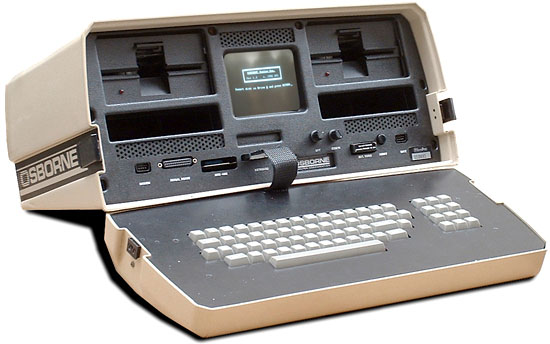
\includegraphics[width=.45\linewidth]{gfx/osborne}} \quad
        \subfloat[GRiD Compass 1101]
        {\label{fig:example-b}%
         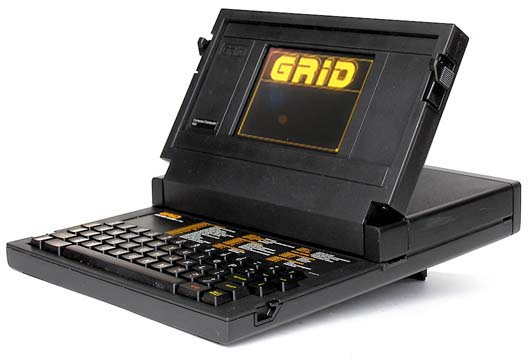
\includegraphics[width=.45\linewidth]{gfx/compass}} \\
        \subfloat[Palm Pilot 1000]
        {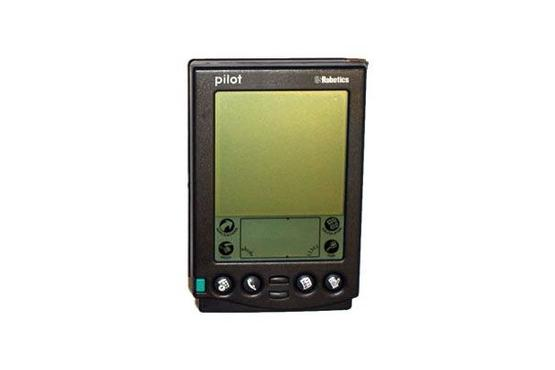
\includegraphics[width=.45\linewidth]{gfx/palm}} \quad
        \subfloat[BlackBerry 5810]
        {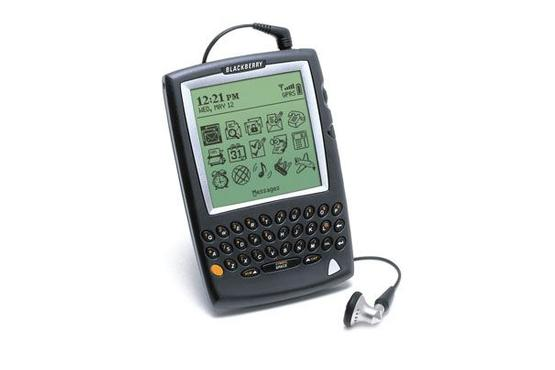
\includegraphics[width=.45\linewidth]{gfx/blackberry}}
        \caption[First mobile computing devices]{First mobile computing devices}\label{fig:example}
\end{figure}
%************************************************
\chapter{Current mobile Platforms}\label{ch:m_plats} % $\mathbb{ZNR}$
%************************************************
\section{Android}
\spacedlowsmallcaps{Android} is a Linux based operating system specially designed for touchscreen devices like smartphones or tablets. It began as the brain-child of a new company called Android, Inc. back in 2003.

\begin{quotation}
Android, Inc. was founded in Palo Alto, California in October 2003 by Andy Rubin (co-founder of Danger), Rich Miner (co-founder of Wildfire Communications, Inc.), Nick Sears (once VP at T-Mobile), and Chris White (headed design and interface development at WebTV) to develop, in Rubin's words "smarter mobile devices that are more aware of its owner's location and preferences". The early intentions of the company were to develop an advanced operating system for digital cameras, when it was realised that the market for the devices was not large enough, and diverted their efforts to producing a smartphone operating system to rival those of Symbian and Windows Mobile (Apple's iPhone had not been released at the time). Despite the past accomplishments of the founders and early employees, Android Inc. operated secretly, revealing only that it was working on software for mobile phones. That same year, Rubin ran out of money. Steve Perlman, a close friend of Rubin, brought him \$10,000 in cash in an envelope and refused a stake in the company.
\cite{wikipedia:android}
\end{quotation}

Google bought Android, Inc. in 2005 and made it a wholly owned subsidiary. The most important employees stayed and started working on what later would become the Android Operating System.

Up until the release of the first Android Device on October \nth{22}, 2008, Google conducted secret meetings with many handset and chip manufacturers to discuss the creation of a new consortium, the Open Handset Alliance, with the goal to develop open standards for mobile devices. The Alliance was unveiled on November \nth{5}, 2007.\footnote{\url{http://www.openhandsetalliance.com/press_110507.html}}


After the first device with Android, the HTC Dream, was released there has been a major surge of devices using Android. Hardware manufacturers from all over the world have chosen Android as their favourite operating system, not only for smartphones and tablets but also for embedded devices like the Cotton Candy Stick from FXI Technologies and even gaming consoles like the Ouya. %They have gone the Android route to give their devices a robust and secure operating system.


The development of system features and other components has been done at a steady pace, releasing new versions of the OS every couple of months. The team has chosen to give colourful names to each release, always in alphabetical order and always named after a dessert or a sweet treat. A closer look at \autoref{fig:android1} and \autoref{fig:android2} should give you  better overview over the different versions of Android and what each new version brought forth.   

\begin{figure}
    \hbox{
        \hspace{-4em}
        {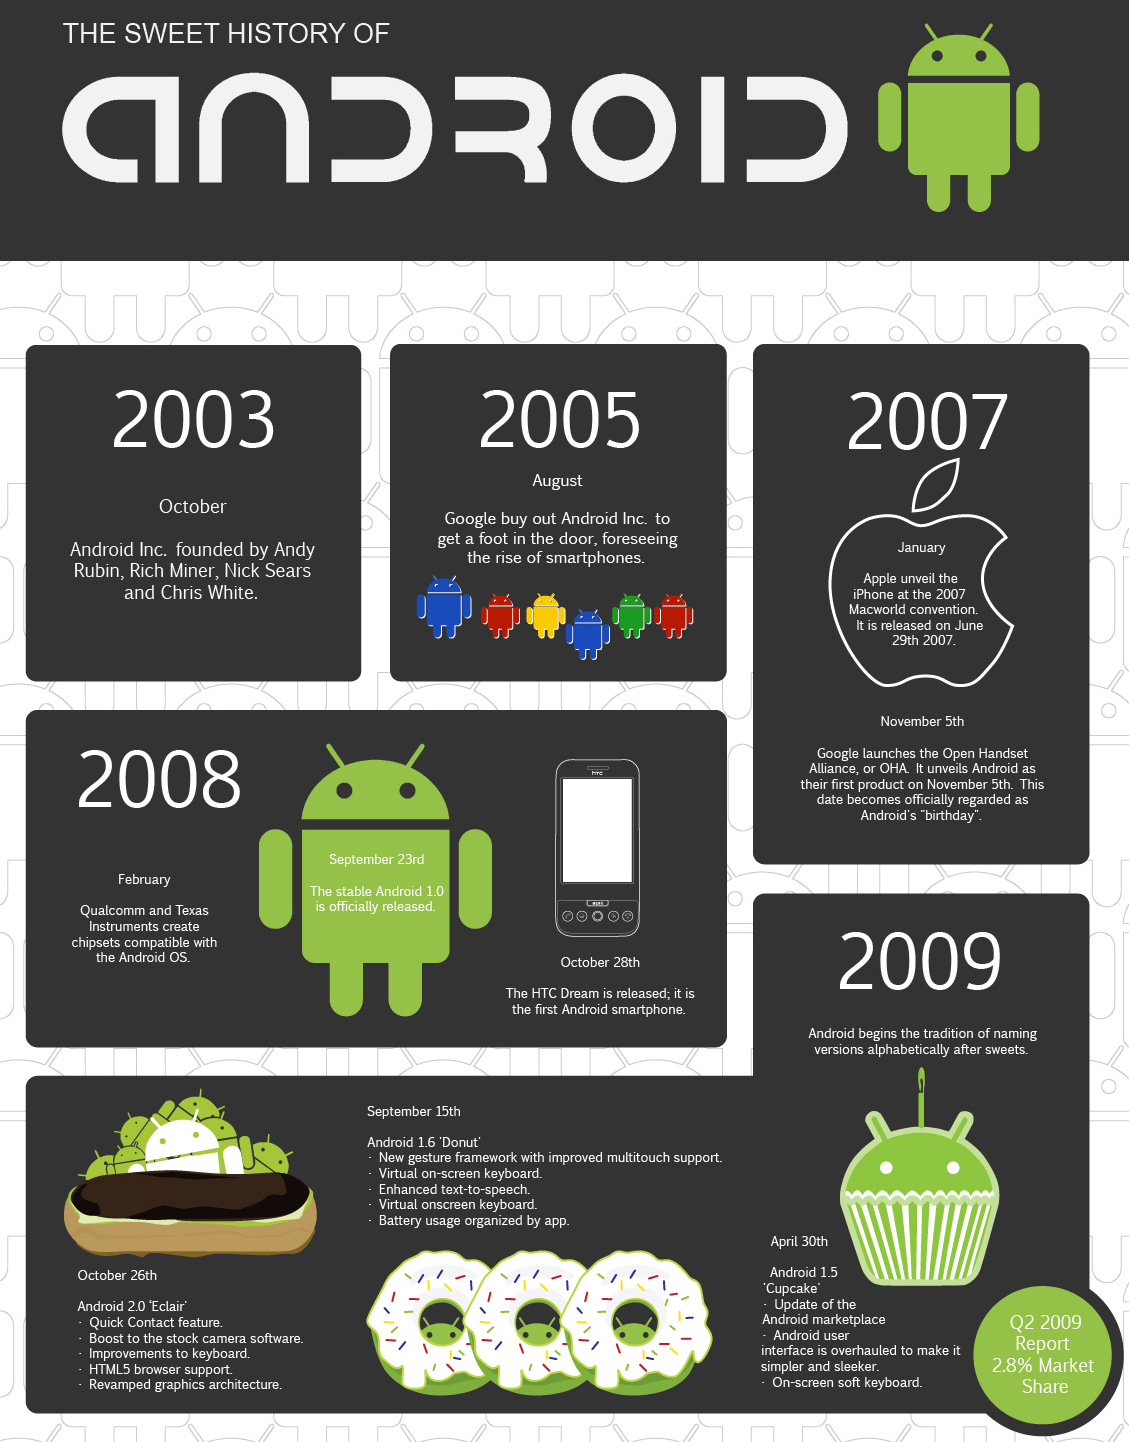
\includegraphics[width=1.5\linewidth]{gfx/android-history1}}
        \caption[Visual History of Android, Part 1]{Visual History of Android}\label{fig:android1}
    }
\end{figure}
\begin{figure}
    \hbox{
        \hspace{-12em}
        {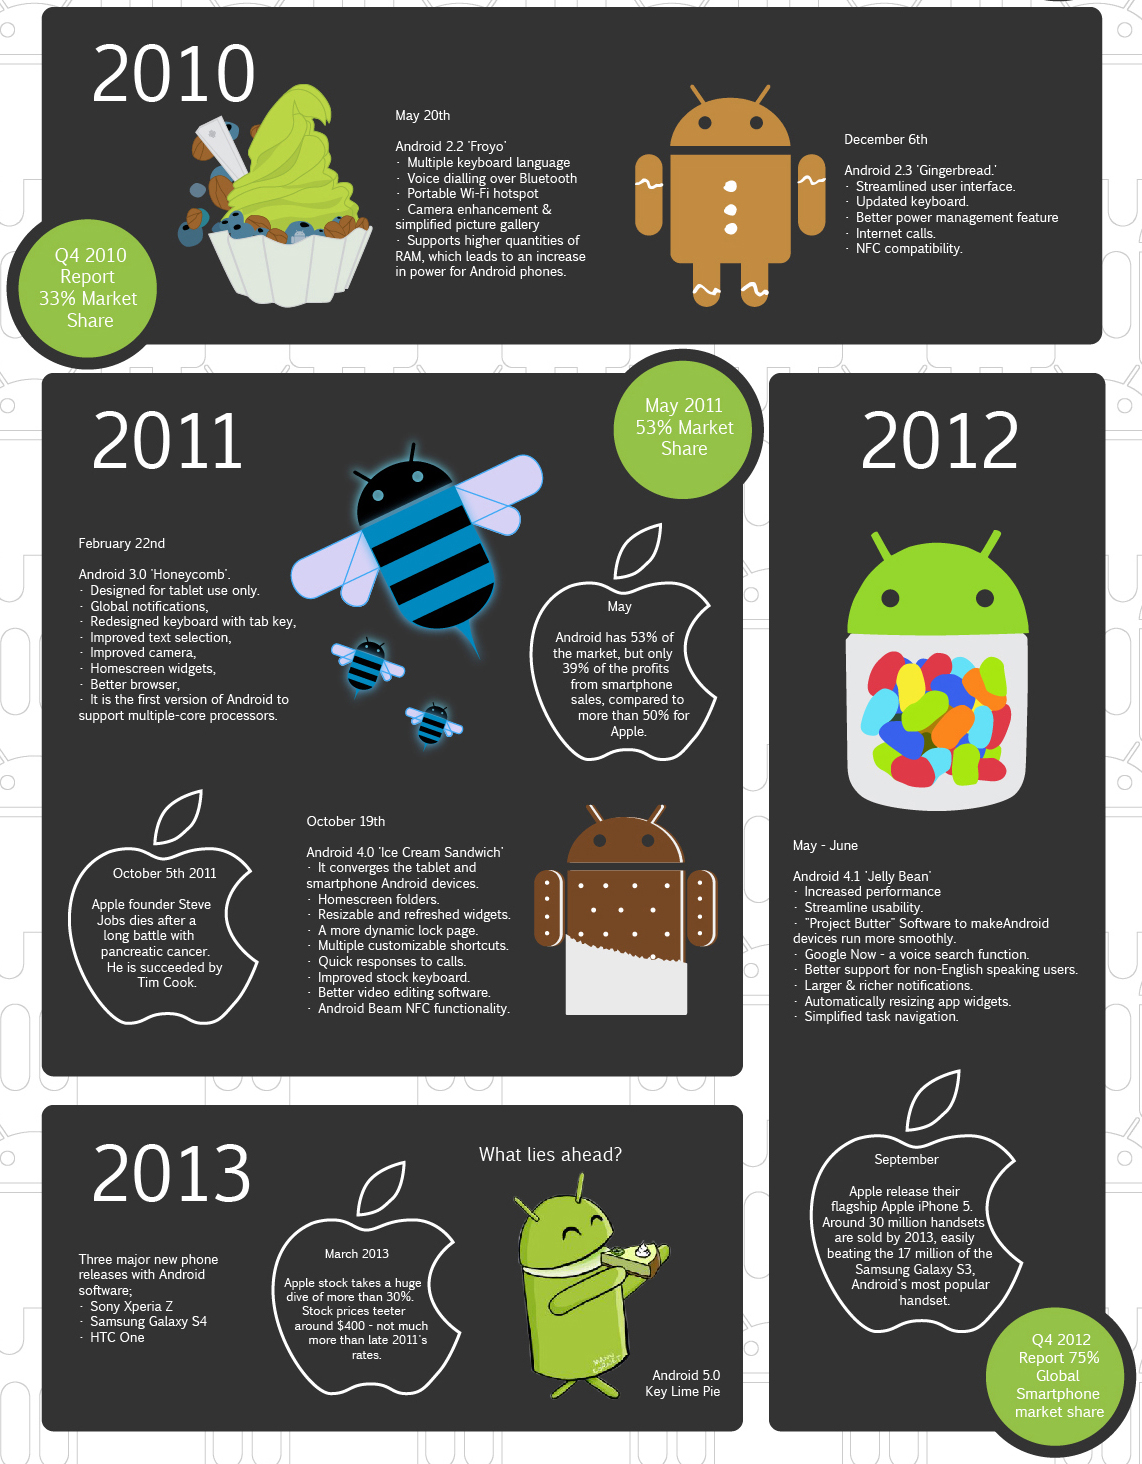
\includegraphics[width=1.55\linewidth]{gfx/android-history2}}
        \caption[Visual History of Android, Part 2]{Visual History of Android\footnotemark}\label{fig:android2}
    }
\end{figure}
\footnotetext{Source: \url{http://visual.ly/sweet-history-android}}\\

\subsection{The Android Open Source Project}
One of the best features and assets of Android is that it is 100\% Open Source. This allows everyone with the necessary knowledge to contribute to the development of the platform and also to modify it in every way you want.


This is exactly what the guys behind CyanogenMod have done. They took the regular Android Operating System and added many features and improvements to the core experience, making it the most popular unofficial Android OS.


But these types of modifications are not only common inside hobbyist communities, big corporations also contribute code to the Android Project. Some even modify the code so much, that it becomes almost unrecognisable. That is exactly what Amazon did. They took the Android OS and heavily modified it in order to install it in their Kindle Fire family of tablets.


Using an Open Source Model also guarantees Android an independent future from Google. Even if Google stops supporting \marginpar{Note: Google is unlikely to stop supporting Android} Android, the community will pick up the pieces and continue with its development and will guarantee its longevity.
 
\section{BlackBerry}
\section{iOS}
\begin{figure}[H]
    \begin{center}
        {\includegraphics[width=.90\linewidth]{gfx/ios-history}}
        \caption[Visual History of iOS]{Visual History of iOS\footnotemark}\label{fig:ios}
    \end{center}
\end{figure}
\footnotetext{Source: \url{http://visual.ly/history-ios}}\\

\section{Windows Phone}
\section{Other platforms worth noting}
The platforms mentioned above are the most popular ones. Together they control around 95\% of the mobile market, however, there are companies like Mozilla and Cononical that want to enter the competition and bring forth completely new ideas on what a mobile operating system should be.

\subsection{Firefox OS}
\spacedlowsmallcaps{Firefox OS} is Mozilla's entry to the mobile market. It hopes to revolutionise the mobile ecosystem by proposing that all applications for the device be programmed using Web Technologies.

\begin{quotation}
On July 25, 2011, Dr. Andreas Gal, Director of Research at Mozilla Corporation, announced the "Boot to Gecko" Project (B2G) on the mozilla.dev.platform mailing list. The project proposal was to "pursue the goal of building a complete, standalone operating system for the open web" in order to "find the gaps that keep web developers from being able to build apps that are – in every way – the equals of native apps built for the iPhone [iOS], Android, and WP7 [Windows Phone 7]." The announcement identified these work areas: new web APIs to expose device and OS capabilities such as telephone and camera, a privilege model to safely expose these to web pages, applications to prove these capabilities, and low-level code to boot on an Android-compatible device.
This led to much blog coverage. According to Ars Technica, "Mozilla says that B2G is motivated by a desire to demonstrate that the standards-based open Web has the potential to be a competitive alternative to the existing single-vendor application development stacks offered by the dominant mobile operating systems."
\cite{wikipedia:firefox}
\end{quotation}

In 2012 B2G was rebranded as Firefox OS in honour of the company's flagship product, the Firefox Web Browser.


Some preview units have been shipped to journalists and developers, in order to gain some traction, but the system has not come to production, yet. 

\begin{quotation}
In February 2013, Mozilla announced plans for global commercial roll-out of Firefox OS. Mozilla announced at a press conference before the start of Mobile World Congress in Barcelona that the first wave of Firefox OS devices will be available to consumers in Brazil, Colombia, Hungary, Mexico, Montenegro, Poland, Serbia, Spain and Venezuela. Firefox have also announced that LG Electronics, ZTE, Huawei and TCL Corporation have committed to making Firefox OS devices.
\cite{wikipedia:firefox}
\end{quotation}

 

\subsection{Ubuntu Phone}
\spacedlowsmallcaps{Ubuntu Phone} is Conical's horse in the mobile race. With it, Canonical hopes to disturb the mobile market by offering a single operating system capable of being a Mobile OS and a Desktop OS. As Canonical's own website puts it, 

\begin{quotation}
High-end smartphones have a brain as powerful as ultra-light laptops. Ubuntu uniquely enables a new category of convergence device – phones that dock to become full PCs and thin clients; enabling enterprise IT departments to replace phones, thin clients and laptops with a single secure corporate device.\\

Operators targeting the enterprise market with LTE can now deliver a full laptop/phone solution, with Windows apps delivered over LTE from the corporate data center. And operators in emerging markets can deliver desktop applications to the converged device over LTE as a premium data service.\footnote{\url{http://www.ubuntu.com/phone/operators-and-oems}}
\end{quotation}


\spacedlowsmallcaps{Ubuntu Phone} is still in the early stages of development, but has already gained the backing of major OEM's and carriers around the world. Once it hits the market, it will become the next player to watch, doubtlessly bringing new ideas and features to the table.  
















 
\cleardoublepage
\ctparttext{}
\part{Developing multi-platform applications}
%************************************************
\chapter{Frameworks for multi-platform development}\label{ch:frameworks}
%************************************************
There are numerous frameworks that have been developed over the years to facilitate the creation of multi-platform applications. Just like in the 90s, when vendors saw market opportunities in releasing multi-platform applications for the desktop, most of the solutions available for cross-platform mobile development are of the commercial nature.


However, \marginpar{PhoneGap is the commercial name of the Apache Cordova Open Source Project.} some open source players do exist. They have been gaining popularity and better features over time, some have even been backed by bigger organisations, and now offer both free and commercial packages. Examples worth noting in this category are PhoneGap, backed by Adobe and MonoTouch, backed by Xamarin.
\graffito{Mono is an open source implementation of Microsoft's .NET Framework.}

\section{Types of Frameworks}
When it comes to choosing the adequate framework to use for the development of your application, there are many options that vary in number of features, pricing and support; but they can all be sorted into three distinct categories, based on the type of application they produce at the end. These categories are:
\begin{enumerate}
    \item HTML5 Web Applications (\autoref{sec:web_app})
    \item Hybrid Applications (\autoref{sec:hyb_app})
    \item Pseudo-Native Applications (\autoref{sec:pseudo_app})
\end{enumerate}

You should always keep in mind the advantages and drawbacks of each when choosing which type of framework is the best for your needs, but let us take a look at \autoref{tab:frameworks} first. It should give you an overview over the technologies used and the type of applications produced by the most popular cross-platform frameworks. We will discuss each type in detail later on.\newline

\begin{table}[H]
    \myfloatalign
  \begin{tabularx}{\textwidth}{Xll} \toprule
    \tableheadline{Name} & \tableheadline{Language} & \tableheadline{Type}\\ 
    \midrule
    Any web framework & HTML5 \& Javascript & Web App\\
    Corona SDK & Lua & Pseudo-Native\\
    Embarcadero & Delphi \& C++ & Pseudo-Native\\
    Icenium\textsuperscript{*} & Javascript & Hybrid\\
    Intel XDK\textsuperscript{*} & Javascript & Hybrid\\
    PhoneGap\textsuperscript{*} & Javascript & Hybrid\\
    Rhodes & Ruby \& Javascript & Hybrid\\
    Titanium SDK & Javascript & Hybrid\\
    Xamarin & C\# + Native UI & Pseudo-Native\\      
    %\midrule
    \bottomrule
  \end{tabularx}
  \caption[Characteristics of the most popular cross-platform frameworks]{Overview of some characteristics of the most popular cross-platform frameworks\footnotemark}  \label{tab:frameworks}
\end{table}
\marginpar{\vbox{\vspace{-24em}\textsuperscript{*} All of these frameworks are based on Apache Cordova}}
\footnotetext{Information taken from the Framework's respective website}  

As \autoref{tab:frameworks} lets us see, the majority of available frameworks seem to be those that deliver a hybrid application. This phenomenon can be explained by what \citeauthor{allen:2010} express in their book about Cross-Platform Development:
\begin{quotation}
The innovation in cross-platform frameworks for smartphone applications surpasses the patterns of abstraction seen in the cross-platform desktop frameworks of the 1990s. These new smartphone frameworks are influenced by the rapid application development techniques we are seeing in web development today. There are three specific techniques in web application development that are borrowed for these non-web frameworks: 1) layout with mark-up (HTML/CSS); 2) using URLs to identify screen layouts and visual state; and 3) incorporating dynamic languages, such as Javascript and Ruby.\\

A generation of designers and user interface developers are fluent in HTML and CSS for layout and construction of visual elements. Additionally, addressing each screen by a unique name in a sensible hierarchy (URL) with a systemized way of defining connections between them (links and form posts) has created a lingua franca understood by visual and interactions designers, information architects, and programmers alike. This common language and its standard implementation patterns led to the development of frameworks and libraries that significantly speed application development on the Web. These patterns are now being applied to the development of mobile applications as common techniques by individual developers as well as in cross-platform frameworks.
\cite[p. 23]{allen:2010}
\end{quotation}
Before we dive into each type of framework, \autoref{fig:hybrid_native} should give you a better overview over their capabilities.\\

\marginpar{\autoref{fig:hybrid_native}: The 'Native' label also applies to Pseudo-Native}
\begin{figure}[H]
    \begin{center}
        {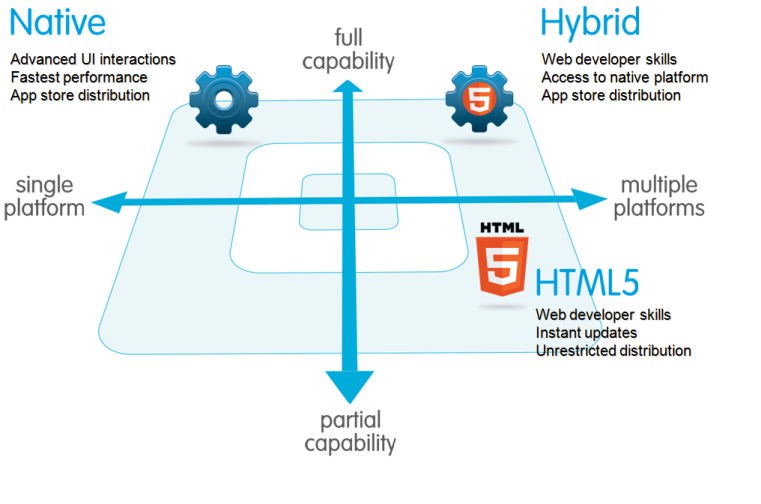
\includegraphics[width=1\linewidth]{gfx/Native_html5_hybrid}}
        \caption[Overview of app capabilities. Native vs. Hybrid vs. HTML5]{Overview of app capabilities. Native vs. Hybrid vs. HTML5\footnotemark}\label{fig:hybrid_native}
    \end{center}
\end{figure}
\footnotetext{Source: \url{http://wiki.developerforce.com/page/Native,_HTML5,_or_Hybrid:_Understanding_Your_Mobile_Application_Development_Options}}\\

\subsection{HTML5 Web Applications}\label{sec:web_app}
Just as any other website, \spacedlowsmallcaps{HTML5 Web Applications} can be developed in any language that can be translated to HTML code on runtime. Some examples of these languages are \emph{Ruby, PHP, Python, JSP} or just plain HTML. Some of the most popular web development frameworks, like Ruby on Rails or Synfony\marginpar{Synfony is an MVC Framework for PHP, similar, but not quite as powerful as Rails.}, are very well suited for the development of Web Applications for Mobile Devices.


But having HTML code is not everything, you still need to make it look good in the smaller screen of cellphones and tablets. That's where CSS3 comes into play. With CSS3 you define the look and feel of the application, but you need to define specific rules for devices with a smaller resolution. This can be accomplished in two ways:
\begin{enumerate}
    \item Responsive CSS3 Design
    \item Separate Domain and CSS files for mobile devices
\end{enumerate}
\spacedlowsmallcaps{Responsive CSS3 Design} means you need to distinguish between the different screen sizes and define different rules and properties for each inside your CSS files. With responsive design, changes in screen orientation can also be translated to a different layout, e.g. changing the width of tables or the arrangement of images.


With \spacedlowsmallcaps{Separate Files} you will have to redirect visitors using a mobile device to a different domain and have that domain serve the corresponding CSS files. This approach has some caveats, the most obvious one being the overhead of a different domain with separate HTML and CSS files to maintain and the fact that if you want your layout to react to screen dimension changes, you will most likely need to implement some sort of responsive design, anyway.   
 

These frameworks, however, cannot run inside the mobile device; they need to run on a server, which means that the only way to access the application is through a web browser.


This line of action is best suited for smaller projects that want to present their website or web application in a better way to mobile users, but don't have the resources to hire a full time application developer. They can use the designer they have at hand and just optimise their online presence for portable devices.

\subsection{Hybrid Applications}\label{sec:hyb_app}
\begin{quotation}
Before any cross-platform frameworks existed, many developers found that embedding Web UI in a native application was a practical way to develop mobile applications quickly and make cross-platform applications easier to maintain. The user interface for mobile applications tends to be presented as a series of screens. From a high level, the mobile UI can be thought of as having the same flow-of-control as a traditional web site or web application. \cite[p. 28]{allen:2010}
\end{quotation}

\spacedlowsmallcaps{Hybrid Applications} are, in a lot aspects, very similar to HTML5 Web Applications. Both rely on HTML, Javascript and CSS for the definition of the UI, but the edge of Hybrid Applications lies in the way they are packaged.


With \spacedlowsmallcaps{Hybrid Applications} the HTML, et al. are contained within a native application, that allows the framework's API to communicate with the operating system, thus leveraging most of the native features the hardware has to offer, e.g. access to the camera, the accelerometer, the GPS, local storage, etc. Access to these features is accomplished via a wrapper that is programmed in each platform's native language and exposes specific methods to an API that is accessible from the HTML side using Javascript methods.


By having access to these features, Hybrid Applications can behave like native applications and, since they are contained within a native package, there is no need for the user to open a web browser. The user never needs to know whether the application is native or hybrid, everything is just one seamless experience. It also gives you the advantage of distributing your application via the platform's store.


This approach gives you many added benefits over a normal HTML5 Application, with little trade-off. There is a learning curve when dealing with the programming frameworks, but the design and layout are still done in HTML and CSS. One of the main benefits you get is that you now have the possibility to make your application available offline and of course the access to system features like push notifications and background services. It is best suited for projects that want to offer more functionality with their mobile applications and are willing to invest some time in learning the new framework.  

\subsection{Pseudo-Native Applications}\label{sec:pseudo_app}
\spacedlowsmallcaps{Pseudo-Native Applications} are completely different from the other two types. They do not rely on HTML for the UI or on Javascript for communication with native features. These applications are compiled to native code and appear to the device as being truly native.


The way the UI is programmed varies between the different frameworks. It can be done using the native tools of each platform; using a visual designer provided by the framework or programatically, using libraries provided by the framework.


Independently from which method is used for the UI, the business logic is always done separately in an effort to abstract as much code as possible, that way you don't need to repeat yourself that much.


One of the downsides of taking this approach, is that you have to program the UI separately for each platform, which translates into more work and somewhat less maintainability. The advantages, however, can offset all the extra effort.


Let's take a look at the advantages offered by this type of applications:

\spacedlowsmallcaps{Speed} By not using any interpreted languages, code performance is increased. This is crucial for applications that need to do a lot of calculations quickly or that rely on the assessment of large amounts of data.

\spacedlowsmallcaps{Flexibility} Since the UI code is not shared between platforms, it gives you the flexibility to adapt and modify the layout of your application depending on which device is running it. It also gives your application a truly native look \& feel and not an emulated one.

\spacedlowsmallcaps{Extra Features} There are some device features that are not available via Wrapper APIs but can be accessed by these frameworks, either by extra libraries or by manually extending the framework with native code. This gives you complete control over what you application is capable of doing.

\spacedlowsmallcaps{Code Reusability} If you have external libraries that you would like to include in your project, but don't want to rewrite them, using one of these frameworks allows you to include your own libraries in your application if they are programmed in C or C++. 


Using this approach is by no means easy. It requires a lot of investment of time and resources, which most often translates into money. But if you want to have complete control over your project, have code that you want to reuse or simply need your application to run at full speed, this is the right line of action for you.
%************************************************
\chapter{Evaluation of possible frameworks}\label{ch:evaluation}
%************************************************

There are many developers that are happy with just using HTML \& CSS to style their applications and speed up development, but I believe that a mobile application must be true to the platform it runs on. You can try to emulate native \ac{UI} elements with CSS, but it is going to take longer than using true native elements. For that reason the type of app that best suits us is a \textsc{Pseudo-Native Application}. 

We want to use the best framework for the development of the Job Portal Aggregator for the MHM eRecruiting Systems, so in this chapter we will discuss two specific frameworks, \emph{Xamarin} and \emph{Titanium}, since each one takes a different approach at creating the \ac{UI} for multi-platform applications and are the most popular.

In order to make an informed decision, we need to evaluate them based on a fixed criteria.

 

Before we begin with what sets each framework apart, let's take a look at the similarities between them.

\begin{description}
\item[Separate UI implementation:] In order to gain a native look \& feel, the implementation is done (Xamarin) or can be done (Titanium) individually for each platform you plan to support.
\item[Compilation:] Both frameworks compile their projects to native code and allow easy distribution to the platform's store.
\item[Pricing:] Both frameworks offer free and paid packages, though they differ greatly in features offered.   
\end{description}


%*******************
\section{Xamarin}
After Novell laid off the entire workforce dedicated to maintaining Mono, the open-source implementation of Microsoft’s .NET development framework, in May 2007 the team decided to start its own company and continue with the development and improvement of Mono. They called this company Xamarin and mere months after its inception, the company became profitable, striking a deal with SUSE, the company holding all the old Novell assets, to obtain all the rights to Mono and provide support to legacy clients using the Mono Development Framework.\footnote{\url{http://gigaom.com/2011/12/12/xamarin-mono/}}

\subsection{Language \& Services}
Xamarin uses C\# as the main programming language, thus leveraging the standard library of C\# and every external library that can run on the .NET Framework.

Xamarin also offers an array of prime components to its Enterprise Customers, offering pre-built packages to make development of large applications easier and faster, such as \ac{UI} controls, themes \& libraries.

 


\subsection{Development Environment \& UI Generation}
Xamarin Studio is the \ac{IDE} provided by Xamarin, Inc. for use with their framework. It is a multi-platform piece of software aimed to ease development and increase performance.

Like many other \ac{IDE}s, it provides the user with autocompletion, code debugging \& inspection, etc.

One of the biggest advantages of Xamarin Studio is that it incorporates a graphical designer for the Android \ac{UI}, allowing the developer to simply drag-and-drop the elements necessary for each view and adding the necessary logic via user-friendly menus. For iOS it offers integration with the graphical designer of Xcode\marginpar{Xcode is Apple's IDE for Mac \& iOS Development}, called XIB Editor. It allows for the same ease of development, when creating iOS Applications. 


%*******************
\section{Titanium}
Titanium is the free offering of Appcelerator for multi-platform mobile development. Appcelerator's website best describes the Titanium ecosystem:
\begin{quotation}
Our ecosystem enables enterprises and independent developers to rapidly create rich, high quality mobile applications to take advantage of the ever changing mobile device and feature landscape.
Spanning icon libraries, UI components, advertising and encryption, our Marketplace includes over 330 modules or extensions to deliver rich, high quality apps much faster than would otherwise be possible.
\footnote{\url{http://www.appcelerator.com/ecosystem/}}
\end{quotation}
 

\subsection{Language \& Services}
Titanium uses Javascript as the main programming language, but it uses a special set of libraries called CommonJS in order to optimise its \ac{API}.

One of the biggest features of Titanium is the possibility of using the Titanium Cloud Services, a Mobile Backend as a Service (MBaaS), offering a fast and easy way to build connected mobile apps. Developers can choose from a library of services such as push notification, status updates, photo storage, and social integration, or create their own custom cloud services.\footnote{\url{http://www.appcelerator.com/cloud/}} 



\subsection{Development Environment \& UI Generation}
Titanium \marginpar{Alloy is an MVC Framework based on Titanium for Hybrid Applications} Studio is the \ac{IDE} provided by Appcelerator for use with their framework. It is a heavily optimised, Eclipse based \ac{IDE} aimed to provide extended features for the Titanium and Alloy Frameworks.

For the development of \ac{UI} elements you can only rely on the different \ac{API} calls provided by the framework. There is no graphical designer, so every change to the layout must be done in code. Titanium does try to simplify this, by placing components that have equivalent counterparts in different platforms within the same namespace.   



%*******************
\section{Putting them to the test}
Now that we know exactly what sets each framework apart and what they do best, we can take a more focused approach at testing each framework according to our requirements.

\begin{itemize}
\item We need our application to comply with German Data Protection Laws, so we need it to provide encryption for personal data and for the database.
\item It needs to efficiently communicate with a cloud service and parse the data received in a timely matter.
\item Development of the application must not take longer than 3 months, so we need to measure how long it takes in average to complete an equivalent application in each of the frameworks.  
\item The code produced at the end needs to be easy to understand and easy to maintain.   
 
  
\end{itemize}



%*******************
\section{Conclusion}

After all the evaluations, we can see that ... adjusts the best to our needs. 




Now that we have chosen the right framework for our endeavour, we can take a look at the next piece of the puzzle. Before we can start with the development of the application, we still need to discuss a very important part of almost all current applications; a connection to the cloud. 

In the next part we will discuss what the cloud actually is, how it comes into play with mobile applications and why are so may companies investing Millions of Dollars in cloud technology. 
%\addtocontents{toc}{\protect\clearpage} % <--- just debug stuff, ignore

\ctparttext{}
\part{The Cloud}
%************************************************
\chapter{Cloud Computing \& The Cloud}\label{ch:infrastructure}
%************************************************
For the past 5 years we have seen the terms "cloud" and "cloud computing" used to describe different services and offers from all around the Internet, but there isn't really a consensus on what the "cloud" really is. So, before we can begin to describe the infrastructure of a Cloud Service, we must first define what the these terms mean and why they are so important to the current IT environment.

\section{Defining the Cloud}
The term "The Cloud" has become a familiar metaphor for the Internet. A lot of people simply refer to everything that is outside of a firewall as "the cloud", but it isn't until you combine the term with the word "computing" that it takes on a different meaning. And with this new meaning come different definitions of what the phrase entitles.\footnote{\url{http://www.infoworld.com/d/cloud-computing/what-cloud-computing-really-means-031}}

For most professionals the term "Cloud Computing" is a synonym for Distributed Computing over a Network. Distributed Computing means the ability to run a computer program on many machines at the same time, thus distributing the working load over all of these machines' processors.\footnote{\url{http://en.wikipedia.org/wiki/Distributed_computing}}

The \ac{NIST} defines Cloud Computing as:
\begin{quotation}
[...] a model for enabling convenient, on-demand network access to a shared pool of configurable computing resources (e.g., networks, servers, storage, applications, and services) that can be rapidly provisioned and released with minimal management effort or service provider interaction.
\footnote{\url{http://www.nist.gov/itl/cloud/upload/cloud-def-v15.pdf}} 
\end{quotation}

This definition makes it clear that Cloud Computing is a model and not a technology, which means there can be many different implementations and variations of the base model, each with its own distinct advantages and disadvantages.

The machines involved in Cloud Computing are usually virtual servers. These virtual servers appear to be, in every sense, real servers, but actually run on a virtual machine that can be scaled up or down depending on the needs of the applications it runs.

So for the purposes of this thesis we will expand on the \ac{NIST} definition of Cloud Computing with the following:
\begin{description}
\item[Cloud:] A distributed network of machines or virtual machines that collaborate within the scope of a given application/service or provide necessary services to said application/service.  
\item[Cloud Computing:] The ability to execute any number of computations on the Cloud, without having to worry about how the data is actually distributed.
\end{description}

Furthermore the term \textsc{Cloud Service} will be given to an application or service that runs on the cloud.

\section{The Infrastructure of the Cloud}

As we described in the previous section, our version of the cloud consists of an array of virtual machines. This array can be hosted on a single physical machine or on several networked machines.

There are many types of virtualization, e. g. Memory, Network, Storage, Hardware and Service Virtualization. The last one encompasses all the previous ones and has been the building block of most of the different Cloud implementations currently available.\footnote{\url{http://www.f5.com/pdf/white-papers/virtualization-defined-wp.pdf}}

It is very interesting that virtualization, the logical abstraction of hardware through a layer of software, has been around, in one way or another, since the mainframe era\cite[p. 3]{williams:2012} and it is now driving a revolution not only in cloud technology and its infrastructure, but also within the Enterprise, allowing businesses to better utilize their IT resources and save money.   

Thanks to the \ac{NIST} definition we also know that cloud computing must be easy to configure, highly accessible, fast to deploy and highly scalable. These are all characteristics of a virtualized system.
\cite{vmware:2007}

There are a few companies that have been pushing the development of virtualization technology, and bringing forth new ideas and improvements to the field. They are \textit{Citrix}, \textit{Microsoft}, \textit{Parallels} and \textit{VMware}.

These companies offer professional virtualization solutions for Enterprises and Individuals looking to build their own cloud infrastructure. Be it on-premises or on a datacenter with rented servers, they offer different products that scale based on the needs of the customer.

A quick look at \autoref{fig:vm} should give you an overview of how virtualization works. 

\begin{figure}[H]
    \begin{center}
        {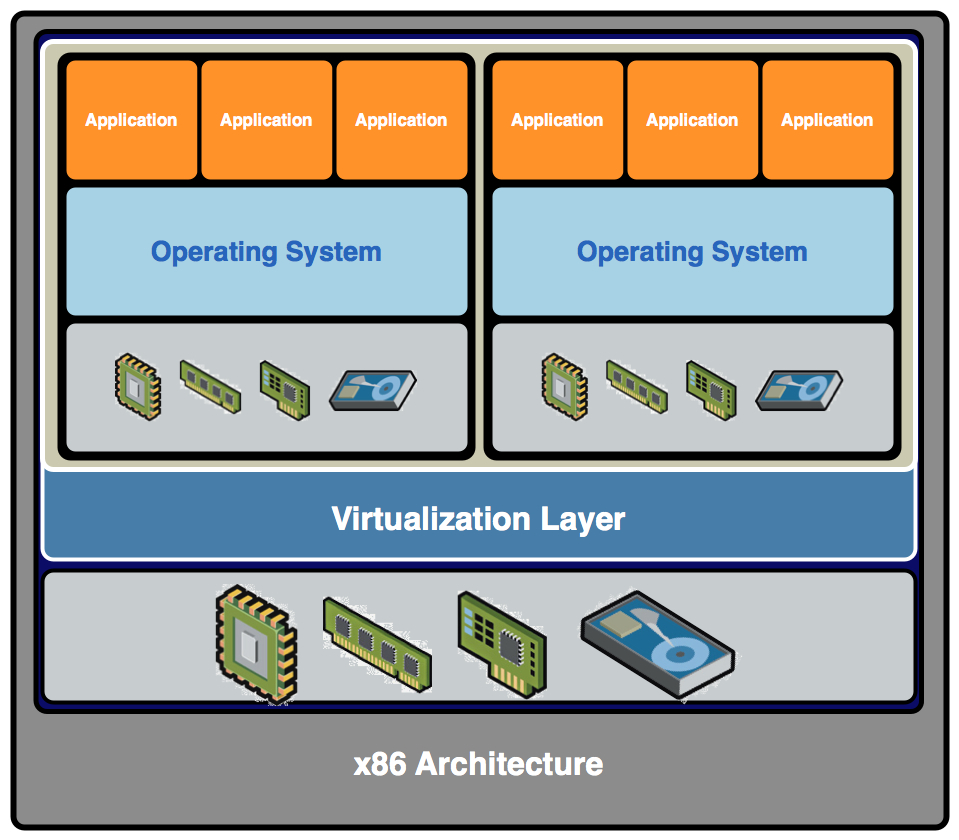
\includegraphics[width=.70\linewidth]{gfx/vm}}
        \caption[Hardware Virtualization]{Hardware Virtualization\footnotemark}\label{fig:vm}
    \end{center}
\end{figure}
\footnotetext{Source: \url{http://www.vmware.com/files/pdf/VMware_paravirtualization.pdf}}\\

Professional Virtualization products are based on one of the three different types of Hardware Virtualization:
\begin{description}
\item[Full Virtualization] uses a combination of direct execution of user requests and binary translation of \ac{OS} requests. It translates kernel code to replace non-virtualizable instructions with new sequences of instructions that have the intended effect on the virtual hardware.

It simplifies migration, portability and scalability of the Guest \ac{OS} and offers the best isolation and security for virtual machines.
\cite[p. 4]{vmware:2007}

\item[Hardware Assisted Virtualization] relies on improvements made by the chip vendors, like Intel and AMD, in order to simplify virtualization techniques.

These improvements target privileged instructions with a new CPU execution mode feature that allows the hypervisor\marginpar{Hypervisor: A software layer in charge of running and managing the virtual machines} to run in a new root mode below the Guest \ac{OS}. Thus, privileged and sensitive calls are automatically trapped by the hypervisor, removing the need for either binary translation or
paravirtualization.
\cite[p. 6]{vmware:2007}

\item[OS Assisted Virtualization/Paravirtualization] It involves modifying the OS kernel to replace non-virtualizable instructions with hypercalls that communicate directly with the virtualization layer hypervisor and its value lies in a smaller overhead.

It is actually easier to modify the Guest \ac{OS} to support Paravirtualization than to build the more sophisticated binary translation support needed for Full Virtualization.
\cite[p. 5]{vmware:2007}
\end{description}


The products of these companies, together with \textsc{QEMU},\marginpar{QEMU is an open source processor emulator and virtualizer that uses full virtualization} provide the infrastructure of most cloud offerings currently available.    

\section{Different Types of Cloud Services}
The breadth of possible applications and services that can run on top of Cloud Technology is astounding, however they can all be classified into three distinct types, \textit{\ac{IaaS}, \ac{PaaS}} and \textit{\ac{SaaS}}. These three types combined are often referred to as \textit{The Cloud Computing Stack} (See \autoref{fig:ipsaas}), but you don't need to be running all of them in order to be using cloud computing.
\cite[p. 8]{mcgrath:2012}  

\begin{description}
\item[Infrastructure as a Service] involves itself with the lowest layer of Cloud Computing, as it provides the components necessary to run any kind of application on top of a physical, or (more often) a virtualized infrastructure.

Providers of \ac{IaaS} usually offer their clients everything they need in order to easily manage and configure their service. This includes the capability to provision processing, storage, networks, and other fundamental computing resources that the customer can use to run any kind of software, including operating systems and applications. 

The provider manages and controls the underlying cloud infrastructure and the user has control over the operating systems, storage and deployed applications.
\cite[p. 8]{sabharwal:2013}

Some examples of \ac{IaaS} Providers include \textit{Amazon}, with its Elastic Cloud service\footnote{\url{http://aws.amazon.com/ec2/}}; \textit{ Microsoft}, with Windows Azure\footnote{\url{http://www.windowsazure.com/}}; \textit{VMware}, with its vCloud Hybrid\footnote{\url{http://vcloud.vmware.com/}} service and \textit{DigitalOcean}\footnote{\url{https://www.digitalocean.com/}}.
 
\item[Platform as a Service] lays in the middle of the Cloud Computing stack and sits right on top of an already defined infrastructure. With this kind of service, the infrastructure is completely managed by the provider; this means that the customer doesn't need to care about the \ac{OS}, storage or networks and can focus all its resources on the application itself.
\cite[p. 9]{mcgrath:2012}

A proper \ac{PaaS} provider takes care of everything needed to run some specific language or technology stack. A great example of this is \textit{Heroku}\footnote{\url{https://www.heroku.com}}. It allows you to easily deploy any \textit{Ruby on Rails} Application in a couple of minutes and provides everything you need to manage it and increase its resources.

\item[Software as a Service] is the last layer of the Cloud Stack. This layer provides a full application to the end user in the form of a service. The end user has access to this software through a thin client interface such as a web browser. 

The provider manages the underlying cloud infrastructure such as network, servers, \ac{OS}, storage, and even individual application capabilities but the client may have some control over the application configurations and settings.
\cite[p. 9]{sabharwal:2013}

The best examples of \ac{SaaS} Applications are all of Google Services. You use Gmail or Google Drive without worrying about software updates or how the underlying infrastructure and platform work, you just use the service.
\end{description}

\begin{figure}[H]
    \begin{center}
        {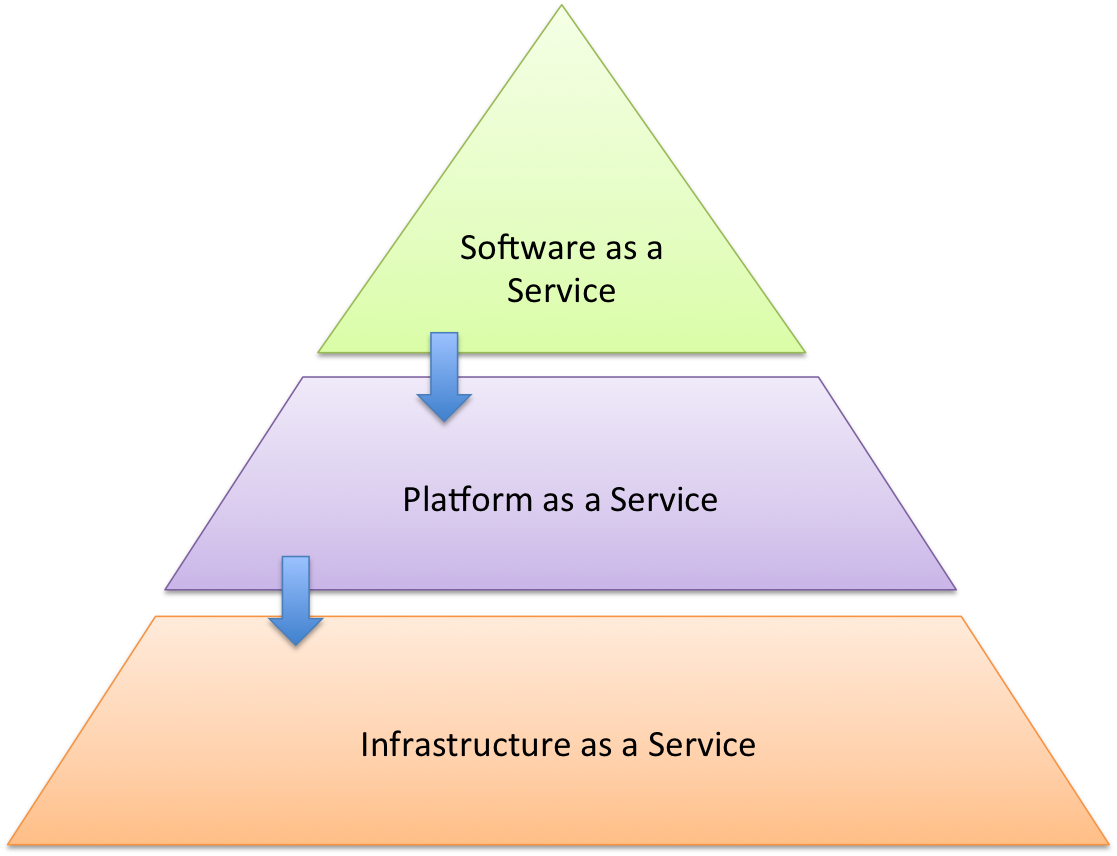
\includegraphics[width=.85\linewidth]{gfx/ipsaas}}
        \caption[The Cloud Computing Stack]{The Cloud Computing Stack}\label{fig:ipsaas}
    \end{center}
\end{figure}

For our purpose, the most important layer is the \ac{SaaS} layer. We want to connect to a cloud application that will provide us with the latest information and status of an already stablished service and allow us to interact with this information.

\section{Significance for Businesses}
Cloud technology is changing the way a lot of companies do business. Now, instead of expending thousands of dollars on server equipment and fiber networks, they can build their infrastructure on the cloud and scale the size of said infrastructure as needed. \cite{williams:2012}

Before the cloud became easily available, companies had to include more space and resources in their infrastructures than actually needed, in order to be able to handle unexpected growth periods.

Knowing how to get this balance right can be very tricky, though. If you include too little overhead and your service grows rapidly, the growth can overwhelm the service and stop it from becoming even greater. But if you plan for a lot of growth and invest a lot of money in extra infrastructure and the service never really takes off, the extra money spent on servers and bandwidth can bankrupt a small company.

This is all a thing of the past, thanks to scalability and high availability of cloud infrastructures. Using cloud technology to build your infrastructure will actually save you money, so a lot of companies are ditching their local infrastructure and upgrading to cloud technology.

This growth in the market has seen an increase in companies offering cloud infrastructure for rent. One of the biggest providers of \ac{IaaS} is Amazon, an online retailer. The fact that an online retailer has a bigger market share\footnote{\url{http://arstechnica.com/information-technology/2013/03/vmware-targets-rival-bookseller-amazon-with-its-own-public-cloud/}} in \ac{IaaS} than tech giants such as Microsoft and VMware, has baffled the industry and was the moving force behind the continuous investment these companies have made in the past year in order to offer the same kind of service and regain all the market they lost.\footnote{\url{http://arstechnica.com/information-technology/2013/08/amazon-and-microsoft-beware-vmware-cloud-is-more-ambitious-than-we-thought/}} 

\section{Influence of the Cloud in Mobile Applications}
The Cloud has had a big impact and influence on how mobile applications have evolved and changed over the past few years. Before the introduction of the Cloud we know today, mobile applications were fairly simple and often focused on productivity and personal organization. The first \ac{PDA} devices did just that. They came with a set of applications developed by the manufacturer and the user could not change the installed applications or add new ones. 

With the dawn of the mobile internet a new wave devices came that were capable of more that just productivity apps. The first applications to be connected to external services were E-Mail and Calendar. This choices were pretty obvious, since they rely on external and up-to-date data.

After mobile internet became faster and more ubiquitous, a new breed of applications started to emerge, applications that relied more and more on data retrieved from remote sources.

This has been the influence of the Cloud on mobile applications. Nowadays it is really hard to find a piece of mobile software that doesn't rely on or offer some kind of Cloud connectivity.  

The many aspects of the cloud, like ease of access, availability, ease of development and low entry cost have changed the mobile landscape and shaped it into what we all use now. Thanks to these technologies, mobile computing is going to continue to evolve and change for the better.





    






%************************************************
\chapter{Connecting to a Cloud Service}\label{ch:introduction}
%************************************************

\ctparttext{}
\part{A real world approach}
%************************************************
\chapter{The MHM Cloud Infrastructure}\label{ch:our_cloud}
%************************************************

Now that we have the perfect communication channels, and before we dive into the development of the multi-platform application, let us take a look at the backend infrastructure that will run our Cloud Service.

We have a \textit{Ruby on Rails API} server set up as the backend for our application. This server is in charge of managing, collecting and updating the current Publications from the different clients of \textit{MHM} that use the eRecruiting application, and has a web front-end where we can manage the companies, add new ones and delete or edit the old ones.

We decided to let a separate server handle and organize the different Publications, because it saves us computing power and gives us a way to expand the apps content without having to publish a new version. Doing everything directly on the app, would require a lot of different connections and would take far longer than what's acceptable.

The server is also necessary for the remote search functionality and the management of certain functions that we will discuss on the upcoming chapters.

In order to keep all Publications up to date, the server connects every hour to all the registered Client eRecruiting Applications, one at a time, and collects information about the available Publications. This is accomplished through an \ac{XML} interface provided the eRecruiting System that collects all valid Publications and lists them as an \ac{XML} file.

The \ac{API} server then uses this \ac{XML} file to gather information about which Publications are new and which ones have been edited, so that it can perform actions on its database accordingly. The diagram in \autoref{fig:api} illustrates how this process works.

\begin{figure}[bth]
    \begin{center}
        {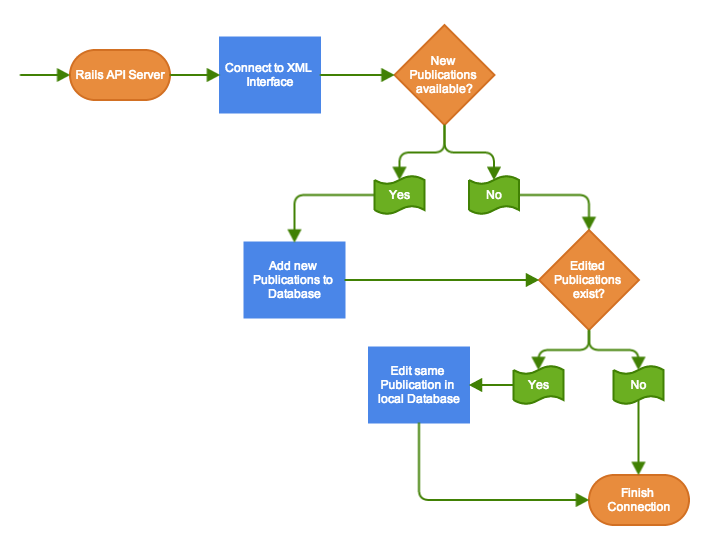
\includegraphics[width=1\linewidth]{gfx/api_flow}}
        \caption[Rails API Workflow]{Rails API Workflow}\label{fig:api}
    \end{center}
\end{figure}

Once the server is done updating the Publications, it is ready to accept incoming connections via its \ac{XML} and \ac{JSON} \ac{API}. The Rails Application exposes different methods for the different actions available to the mobile application. When one of this methods is called, the server performs a query with the database in order to find the matching Publications. It then builds an \ac{XML} or \ac{JSON} file containing all the returned Publications and sends it back to the calling agent.\\
\newline

The methods available to the mobile application are:
\begin{itemize}
\item Get available companies (\texttt{get\_companies})
\item Get the last 100 Job Publications (\texttt{get\_latest\_publications})
\item Send search parameters (\texttt{perform\_search})
\item Save unique device identifier (\texttt{save\_device\_token})
\item Save past searches (\texttt{save\_search})
\end{itemize}

The last two methods available are necessary for the implementation of push notifications. We will discuss this topic in further detail in \autoref{ch:building} and \autoref{ch:passive_com}.

Since almost all of the data management will be done inside the Rails Application, the mobile application doesn't need to keep track of old and new Publications. It can simply drop everything it has once the new data has been received and save this data to its local database, so that it i remains available, even if the user looses internet connectivity.

Now that we have an idea of how the \textit{MHM Cloud Backend} works and connects to the different eRecruiting Systems, let's dive right into the actual development of the MHM Job Portal Aggregator.





%************************************************
\chapter{Building blocks of a cross-platform Application}\label{ch:building}
%************************************************

When building a cross-platform applications, there are many aspects you need to plan, well before you start writing code. Thankfully we already know which framework we are going to use and are familiar with the programming language it uses. 

What we need to do now is analyze the requirements of the application, separate the business logic from the \ac{UI} logic, analyze third-party libraries that may speed up development and implement the application.


\section{Requirements for the MHM Job Portal Aggregator}
Every application needs a purpose. The main purpose of the \ac{JPA} is to consolidate open job vacancies from different sources into an easy to use mobile application. In order to fulfill this, we need to define some requirements of the functionality that the application should offer.  

\begin{description}
\item[Latest Jobs] The main window of the application should show the latest available vacancies, organized in a table view. Each cell should show the title of the vacancy, along with a short description and a small icon depicting the company from where the vacancy came.
\item[Detailed Description] A detailed description of the vacancy should appear when the user clicks on one of the table items. This view should include all the information about the job offering, including salary, benefits and how to apply.
\item[Offline Access] If there is no connection to the internet, the user should still be able to see the vacancies that were loaded the last time the application was opened.
\item[Social Integration] From the detailed description view, the user should be able to share a job offering with his friends via popular social networks like Facebook, Twitter or LinkedIn. 
\item[Search Functionality] Users should be able to search for vacancies based on keywords they enter on the search view. The results should be loaded every time the user changes the search string and the table view should be updated with the new results.
\item[Filters] Pre-defined filters should aid in the navigation of the available job offers.
\item[Saved Searches] The user should be able to save past searches and access them quickly at any time.   
\item[Notifications] The user can opt to receive notifications whenever a new vacancy matching previous searches is posted.
\end{description}

These are the basic requirements to get a functional application that is both useful and easy to use.

\autoref{fig:app_flow} on the following page shows a more detailed view of how the application workflow is supposed to work.

\begin{figure}
    \begin{center}
        {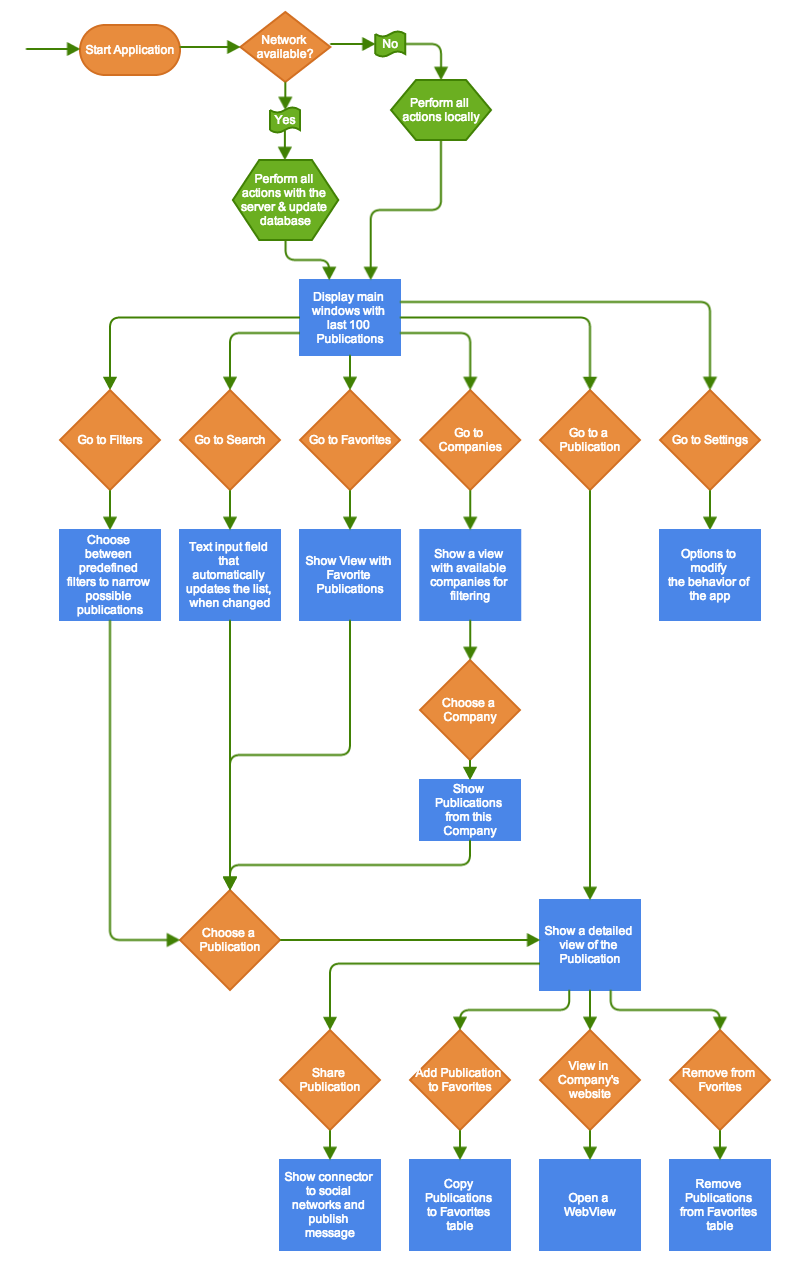
\includegraphics[width=1.14\linewidth]{gfx/app_flow}}
        \caption[Application Workflow]{Application Workflow}\label{fig:app_flow}
    \end{center}
\end{figure}



\section{Platform-Independent Functionality}

The building blocks of any application are mostly located within the business logic, even more so for cross-platform applications, since this is the layer where the shared code resides.

\subsection{Object Models \& Database Connections}
One of the easiest things to share between the platforms is the data handling code. There are two models we need in our application, \texttt{Publication} and \texttt{Company}.  

\texttt{Publications} represent each open vacancy that the application receives from the server and \texttt{Companies} represent each company offering those job applications and are there to help navigate the publications and filter them.

These objects not only represent an instance of the corresponding object in-memory, but, thanks to a third-party library called \textit{SQLite.NET}, they also represent the foundation of an \ac{ORM} System, that makes the creation and management of a local database much easier.

Normally, when using the platform specific SQLite implementation, you need to define the database, insert each element in the table and manage queries and updates manually. 

This can be really cumbersome if you have a lot of tables and elements in your database. By using \textit{SQLite.NET} there is no need for all these formalities, since the 'dirty' work is done by the library itself.
\vfill

\lstset{language=[Sharp]C}
\begin{lstlisting}[frame=lt,caption=Company.cs, label={list:comp}]
using SQLite;
namespace MHMBase
{
	[Table("companies")]
	public class Company
	{
		[PrimaryKey, AutoIncrement]
		public int Id { get; set; }
		[MaxLength(20)]
		public string Name { get; set; }
		public string FullName { get; set; }
		public string IconPath { get; set; }
		public string IconUrl { get; set; }
	}
}
\end{lstlisting}

\begin{lstlisting}[frame=lt,caption=Publication.cs, label={list:pub}]
using SQLite;
namespace MHMBase
{
	[Table ("publications")]
	public class Publication
	{
		[PrimaryKey, AutoIncrement]
		public int Id { get; set; }
		public string RemoteId { get; set; }
		[Indexed]
		public int CompanyId { get; set; }
		public string Title { get; set; }
		public string FullDescription { get; set; }
		public string Company { get; set; }
		[Unique]
		public string Link { get; set; }
		public string ShortDescription { get; set; }
		public bool Favorited { get; set; }
	}
}
\end{lstlisting}

\autoref{list:comp} and \autoref{list:pub} show us all the properties that we need for each model, and also give us a first hand look on how easy it is to use \textit{SQLite.NET}. All that is needed for models like this is to include an \texttt{Id} element with the default getters and setters preceded by the 'magic' attributes so often used in C\# that tell the \textit{SQLite.NET} constructors how to save and define each field in the database. 

\texttt{PrimaryKey} defines the following field as the primary entry of the database and \texttt{AutoIncrement} makes it increase in value, every time a new element is saved to the database. You can also specify the name of the table by adding \texttt{Table ("new-table-name")} before declaring the new class. If you don't specify this value, the table name will default to the class name.

There are many other identifiers that will modify this behavior and they share the same name as the normal SQL modifiers. Some of them are \texttt{Unique, MaxLength, Column}, etc. If you have a field that cannot be saved to the database, you can add the \texttt{Ignore} identifier so that \textit{SQLite.NET} will ignore this field when saving the object to the database.

But this is still just the starting point. We still ned to create an SQLite Connection, create the appropriate table for the objects, create a new object and insert it to the database. Thankfully this is a very easy and straightforward process.

\begin{lstlisting}[frame=lt,caption=DatabaseHelper.cs, label={list:db-save}]
using SQLite;
namespace MHMBase
{
	public class DatabaseHelper
	{
		static DatabaseHelper currentInstance;
		readonly SQLiteConnection db;
		public static DatabaseHelper Instance {
			get {
				if (currentInstance == null)
					currentInstance = new DatabaseHelper ();
				return currentInstance;			
			}
		}

		DatabaseHelper () {
			string folder = System.Environment.GetFolderPath (System.Environment.SpecialFolder.Personal);
			db = new SQLiteConnection (System.IO.Path.Combine (folder, "mhm-jpa.db"));		
		}

		public SQLiteConnection Connection {
			get { return db; }		
		}
	}
}
\end{lstlisting}

\autoref{list:db-save} gives us a first hand look of how we handle the Database Integration. The \texttt{DatabaseHelper} Singleton \marginpar{Singleton: Special Class that only allows for a single instance of itself.} is in charge of creating a single instance of an \texttt{SQLiteConnection} that will be used throughout both Android and iOS applications.

This \texttt{SQLiteConnection} instance is responsible for the management of everything related to the database. It is used to create or delete tables; add, edit or delete items; and to perform queries.

\begin{lstlisting}[frame=lt,caption=DB Snippet, label={list:db-snip}]
var db = DatabaseHelper.Instance.Connection;
// Create Companies Table
db.CreateTable<Company>();
// Create Company Object
var company = new Company {
                Name = "SuperComp",
                FullName = "Super Computers Inc.",
                IconPath = Path.Combine (Environment.GetFolderPath (Environment.SpecialFolder.Personal), "SuperComp.png"),
                IconUrl = "http://supercomp.com/icon"
            };
// Insert new element in DB
db.Insert(company);    
\end{lstlisting}

\autoref{list:db-snip} gives us a simple example of how to get the \texttt{SQLiteConnection} instance, create a table that will store \texttt{Company} objects, create a new object and save it to the database.

\begin{lstlisting}[frame=lt,caption=DB Snippet 2, label={list:db-snip2}]
//Get item by ID
var item = db.Get<Company>(3);
//Delete Item by ID
db.Delete<Company>(3);
//Return all objects in table
var allItems = db.Table<Company>();
//Select item via SQL Statement
var sc = db.Query<Company>("SELECT * FROM Companies WHERE Name = ?", "SuperComp");
//Get all items and order by Name
var companies = db.Table<Company>().OrderBy(c => c.Name);
//Update an object after it has been modified
db.Update(item);
\end{lstlisting}

\autoref{list:db-snip2}, on the other hand, shows us how we can access and manipulate existing objects on the database.

If it weren't for \textit{SQLite.NET} all of the code previously shown would be at least 3 times longer and more complex. Thanks to third-party libraries like this, we can keep our code cleaner and easier to maintain. We will discuss more about what third-party libraries we use later on.   

\subsection{Network Communications}
Another aspect of the application that is easy to share between platforms is the network access. We can easily use all the built in functionality of C\#'s standard library under \texttt{System.Net} and take advantage of asynchronous communication and \ac{LINQ} for \ac{XML} and \ac{JSON} parsing.

\begin{lstlisting}[frame=lt,caption=PublicationsParser.cs, label={list:db-pubparse}]
public void UpdatePublications(Action<IList<Publication>> callback, SQLiteConnection db) {
	db.CreateTable<Publication>();
	var client = new WebClient ();
	client.DownloadStringCompleted += (sender, args) => {
		var pubs = XDocument
		.Parse(args.Result)
		.Descendants("publication").Select(item => new Publication {
			RemoteId = item.Element("id").Value,
			Title = item.Element("title").Value,
			[...]
		}).ToList();
		foreach (var p in pubs) {
			try {
				db.Insert (p);
			} catch (SQLiteException){
				Console.WriteLine ("Duplicate detected");
			}				
		}
		callback(GetPublications(db));
	};
	client.DownloadStringAsync (new Uri (_baseUrl));
}
\end{lstlisting}

A deeper look at \autoref{list:db-pubparse} shows that \texttt{UpdatePublications} method is in charge of fetching the latest \texttt{Publications} and updating the database with the new information. Let's break it apart to see exactly how it works.

The method takes two arguments: a callback action to be executed when the asynchronous download finishes and a reference to an \texttt{SQLiteConnection} object that will update the database.

Once the method starts executing it will create a the \texttt{Publication} table if it doesn't exist already and create an instance of a \texttt{WebClient}. The Web Client does all the heavy lifting and takes care of connecting to the server. The connection is done asynchronously, so we need to define the \texttt{DownloadStringCompleted} method that gets executed once the download of data has completed.

Inside this method lives the code that actually takes care of parsing the \ac{XML} file and saving the new Publications to the database. Thanks to \ac{LINQ}, iterating over each element inside the \ac{XML} file is fairly easy. All we need is an \texttt{XDocument} object to parse the results and iterate over the descendants inside the \ac{XML} tree that match the "publication" tag, then the \texttt{Select} method is called for each item passing a lambda function that makes use of this item and creates a new \texttt{Publication} object. Once everything is done, everything gets thrown into a list and saved to the \texttt{pubs} variable. 

Now that we have a list containing \texttt{Publication} objects we can add them to the database. After everything is saved, we can call the \texttt{callback} function passing as argument the \texttt{GetPublications} function that simply retrieves all elements inside the \texttt{Publications} table.

How the \texttt{callback} functions are used and what they do, we will learn later on.

\begin{lstlisting}[frame=lt,caption=CompaniesParser.cs,label={list:db-compparse}]
foreach (var c in companies) {
	try {
		db.Insert (c);
		var webClient = new WebClient();
		var url = new Uri (c.IconUrl);
		var image_bytes = webClient.DownloadData (url);
		string documentsPath = Environment.GetFolderPath (Environment.SpecialFolder.Personal);	
		string localPath = Path.Combine (documentsPath, c.Name+".png");
		Console.WriteLine("localPath:"+localPath);
		File.WriteAllBytes (localPath, image_bytes);		
	} catch (SQLiteException) {
		Console.WriteLine ("Duplicate detected");					
	}
}
\end{lstlisting}

This process for retrieving the available companies is very similar, almost identical, so we will only take a look at the part that is different. Once everything has been downloaded, parsed and stored in a list, we iterate over this list and if the object doesn't exist in the database, we save it and then download an icon for the logo of this company to the internal storage, so that it can be retrieved by each publication belonging to this company. The code for this can be seen in \autoref{list:db-compparse}.

\section{Third-Party Libraries}

As we mentioned before, third-party libraries are a great way of speeding up development, lowering complexity and improving maintainability. We already talked about one of this libraries, \textit{SQLite.NET}, and how we use it in our application. The following are all the libraries we use that are compatible with both platforms. 

\subsection{Newtonsoft JSON}

As the name implies, \textit{Newtonsoft JSON} is a library designed for parsing \ac{JSON} strings. It has built-in support for \ac{LINQ}, making deserialization much simpler and also supports \ac{XML} to \ac{JSON} conversion.

Inside our application we use it to deserialize the returned result string, when the user preforms a search.

Thanks to \ac{LINQ}, the code in charge of deserializing each element is very similar to the \ac{XML} deserialization code.

\begin{lstlisting}[frame=lt,caption=Publication Search,label={list:search}]
public void SendSearchParameters(Action<IList<Publication>> callback, string parameters) {
	var dl = new WebClient();
	dl.Headers.Add("Content-Type","application/json");
	dl.UploadStringCompleted += (sender, e) => {
		var resultJSON = JObject.Parse (e.Result);
		IList<Publication> publications = resultJSON["publications"].Select(item => new Publication	{
			RemoteId = (string)item["id"],
			Title = (string)item["title"],
			[...]				
		}).ToList();
		callback(publications);
	};
	dl.UploadStringAsync (new Uri (_searchUrl), parameters);		
}
\end{lstlisting}

As \autoref{list:search} shows, we again need a \texttt{WebClient} that takes care of uploading the search parameters to the server and that registers an \texttt{UploadStringCompleted} method that gets executed once the uploading has finished.

Once we have the result string, it gets parsed by the \texttt{JObject} class from \textit{Newtonsoft JSON}. This creates a \texttt{JObject} that is composed of a \texttt{Collection} of \texttt{JTokens}, each representing a serialized element of the result string. We can then access each item inside the "publications" token via \ac{LINQ} with the \texttt{Select} function and create a \texttt{Publication} object out of each item. All of these \texttt{Publication} objects get packed in a list and then passed to the \texttt{callback} function.

The \textit{Newtonsoft JSON} library makes the serialization and deserialization of objects easier and faster. If the \ac{JSON} structure matches the structure of a C\# object, this library can deserialize it and create a new object, without the need to manually match each \ac{JSON} element to an object attribute.
 

\subsection{SimpleStorage}
\textit{SimpleStorage} is a very straight forward third-party library that makes the storing of key-value paired data as easy as possible. It exposes a platform-independent \ac{API} that utilizes each platforms's preferences storage, so you don't need to worry about the implementation in each platform and can share your storage saving code between them.

\begin{lstlisting}[frame=lt,caption=SimpleStorage,label={list:store}]
var storage = SimpleStorage.EditGroup("group name");
storage.Put("myKey", "some value");
var value = storage.Get("myKey");
\end{lstlisting}

We use this library to store simple settings and execution states.


\subsection{SQLite.NET}
We already discussed most of the functionality of \textit{SQLite.NET} in a previous section, so there is not that much to talk about, except for some features that we don't use in our application.

\textit{SQLite.NET} features an asynchronous \ac{API} that doesn't block the main thread while running, thus allowing the rest of the application to continue executing as normal, while the SQL request are performed in the background. The functionality of the library remains the same and the only thing that is different are the method signatures. For example, instead of calling \texttt{CreateTable<T>}, you call \texttt{CreateTableAsync<T>} to create a new table, so all that is needed is to add \texttt{Async} at the end of each method call to use the asynchronous \ac{API}.

\textit{SQLite.NET} also has support for transactions. You can execute database operations inside a transaction and, if something were to fail, the database would be rolled back to the point before the transaction started.

You can also create relationships between objects by adding the \texttt{Indexed} attribute to any model. Going from our application we have the \texttt{CompanyId} field in our \texttt{Publication} model with the \texttt{Indexed} attribute. What this does is
















%************************************************
\chapter{Platform Specific Functionality}\label{ch:ui}
%************************************************

Thanks to the framework we chose to use, and the desire to present our application as natively as possible, there exists the need for some platform specific functionality. Most of this functionality has to do with the \ac{UI} and some third-party libraries.

This chapter will be divided in two parts, one for iOS and one for Android. In here we will also discuss all about the \texttt{callback} functions we mentioned earlier. 

\section{Android UI}

The main reason we chose \textit{Xamarin} as the framework for the development of our application is the fact that we can develop the \ac{UI} in a completely independent fashion.

On the Android side of things, this means using specially crafted \ac{XML} files for defining the look of the application. Under Xamarin Studio, we have two options for laying out the content of each view:  We can use the Android Layout Editor to drag and drop elements form a toolbox or we can  directly edit the \ac{XML} source code and change everything manually.

Since most of the application is composed of Lists and Grids, it is actually easier to manually edit the \ac{XML} source code, than to mess around with the visual editor.

\autoref{list:and_xml} and \autoref{fig:and_layout} show both sides of the same file, the source and how it looks inside the Android Layout Editor.

Decribing what each element inside the \ac{XML} file is, how they work and why they work that way is outside the scope of this work. If you need more information about the inner workings of the Android Operating System, please refer to more specific literature.


\lstset{language=XML}
\begin{lstlisting}[frame=lt,caption=Company.axml, label={list:and_xml}]
<?xml version="1.0" encoding="utf-8"?>
<LinearLayout xmlns:android="http://schemas.android.com/apk/res/android"
    android:orientation="vertical"
    android:layout_width="wrap_content"
    android:layout_height="wrap_content">
    <ImageView
        android:src="@android:drawable/ic_menu_gallery"
        android:layout_width="match_parent"
        android:layout_height="match_parent"
        android:padding="5dip"
        android:gravity="center"
        android:id="@+id/company_image" />
    <TextView
        android:id="@+id/Name"
        android:layout_width="match_parent"
        android:layout_height="wrap_content"
        android:ellipsize="end"
        android:singleLine="true"
        android:textAppearance="?android:attr/textAppearanceSmall"
        android:padding="5dip"
        android:gravity="center"
        android:text="Test" />
</LinearLayout>
\end{lstlisting}


\begin{figure}[H]
    \begin{center}
        {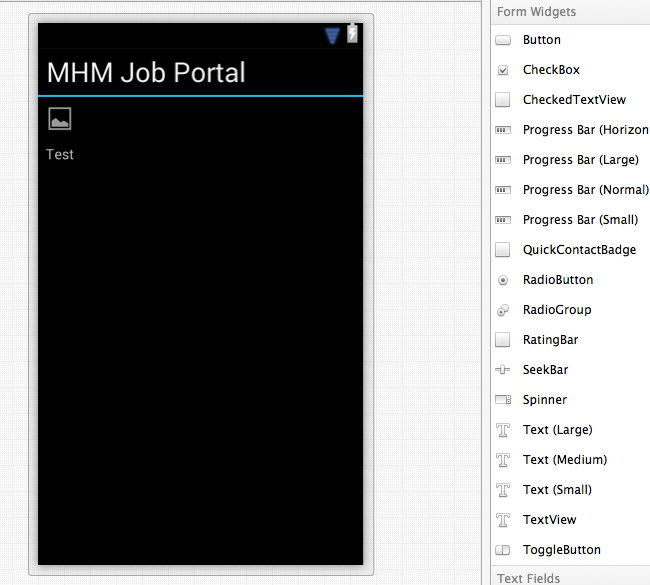
\includegraphics[width=0.75\linewidth]{gfx/and_view}}
        \caption[Android Layout Editor]{Android Layout Editor}\label{fig:and_layout}
    \end{center}
\end{figure}

\subsection{Views, Items and Adapters}
Our Job Portal Aggregator consists of information that is easily packable inside a list, this is why the main view of the application consists of a list of the latest vacancies available.

In order to display this information we need to define a view group where the information will be placed and a view item that represents each element inside the list. All these is done inside the \ac{XML} layout files.

\begin{lstlisting}[frame=lt,caption=Publication.axml, label={list:pub_xml}]
<?xml version="1.0" encoding="utf-8"?>
<LinearLayout xmlns:android="http://schemas.android.com/apk/res/android"
    android:orientation="horizontal"
    android:layout_width="fill_parent"
    android:layout_height="fill_parent">
    <ImageView
        android:src="@android:drawable/ic_menu_gallery"
        android:layout_width="57.2dp"
        android:layout_height="63.0dp"
        android:id="@+id/company_image" />
    <LinearLayout
        android:orientation="vertical"
        android:layout_width="fill_parent"
        android:layout_height="fill_parent">
        <TextView
            android:id="@+id/Title"
            android:layout_width="match_parent"
            android:layout_height="wrap_content"
            android:ellipsize="end"
            android:singleLine="true"
            android:textAppearance="?android:attr/textAppearanceMedium"
            android:padding="5dip"
            android:text="Test" />
        <TextView
            android:id="@+id/Description"
            android:layout_width="match_parent"
            android:layout_height="wrap_content"
            android:padding="5dip"
            android:text="Test" />
    </LinearLayout>
</LinearLayout>
\end{lstlisting}

\autoref{list:pub_xml} describes a Publication element and defines how it will be shown inside the main list. It features the company logo (\texttt{<ImageView>}), the Publication's Title just to the right of the image and its Short Description just bellow the title.

But this is just for one item, we need to define the list that will hold a collection of Publications. In \autoref{list:pubList_xml} we can see that all that is needed is a \texttt{ListView} item. 

\begin{lstlisting}[frame=lt,caption=PublicationsList.axml, label={list:pubList_xml}]
<?xml version="1.0" encoding="utf-8"?>
<LinearLayout xmlns:android="http://schemas.android.com/apk/res/android"
    android:id="@+id/pub_list"
    android:orientation="vertical"
    android:layout_width="fill_parent"
    android:layout_height="fill_parent">
    <ListView
        android:id="@+id/Publications"
        android:layout_width="match_parent"
        android:layout_height="wrap_content" />
</LinearLayout>
\end{lstlisting}

Now that we have defined the list and the appearance of each item within it, we need to connect these elements with real data. That's where adapters come into play. 

\texttt{Adapters} are in charge of populating the list using a collection of items that gets passed via the class constructor. They implement a \texttt{GetView} method that matches elements from the actual object to its visual representation inside the list and define some simple methods for member data accessibility.

\lstset{language=[Sharp]C}

\begin{lstlisting}[frame=lt,caption=PublicationsListAdapter.cs, label={list:pubList_cs}]
class PublicationsListAdapter : BaseAdapter<Publication> {
	readonly LayoutInflater _context; 
	public IList<Publication> Publications { get; set; }

	public PublicationsListAdapter (LayoutInflater context, IList<Publication> publications) {
		_context = context;
		Publications = publications;		
	}

	public override View GetView(int position, View convertView, ViewGroup parent) {
		var view = convertView ?? _context.Inflate(Resource.Layout.Publication, null);
		var pub = Publications[position];
		var db = DatabaseHelper.Instance.Connection;
		var company = db.Table<Company> ().Where (c => c.Name.Equals(pub.Company)).First();
		var imgFile = new File (company.IconPath);
		Bitmap imgBitmap = BitmapFactory.DecodeFile(imgFile.AbsolutePath);
		view.FindViewById<TextView>(Resource.Id.Title).Text = pub.Title; 
		view.FindViewById<TextView> (Resource.Id.Description).Text = pub.ShortDescription;
		view.FindViewById<ImageView> (Resource.Id.company_image).SetImageBitmap (imgBitmap);
		return view; 
	}
}
\end{lstlisting}

Another possibility for displaying a cluster of data is called Grids. They allow you to neatly pack data into what can be considered a two-dimensional list. We use Grids in our application to display the available companies that offer vacant positions.

Grids behave almost identically to Lists. They need an Item Definition, an Adapter and the Grid Definition itself. There is no distinction between adapters and item definitions for lists and their counterparts for grids. The only difference is in how the collections are laid out.

\lstset{language=XML}
\begin{lstlisting}[frame=lt,caption=CompaniesGrid.axml, label={list:grid_xml}]
<GridView xmlns:android="http://schemas.android.com/apk/res/android"
    android:id="@+id/Companies"
    android:layout_width="fill_parent"
    android:layout_height="fill_parent"
    android:columnWidth="120dp"
    android:numColumns="auto_fit"
    android:verticalSpacing="10dp"
    android:horizontalSpacing="10dp"
    android:stretchMode="columnWidth"
    android:gravity="center" />
\end{lstlisting}

This means that the \texttt{CompaniesAdapter} looks exactly the same as the \texttt{PublicationsAdapter}, with the small difference that the collection used is for \texttt{Company} objects. And the \texttt{Company} item has one \texttt{<TextView>} less, because it only needs one for the Company name.
\vfill

\subsection{Activities, Fragments and Navigation}

With the views, items and adapters we have everything necessary to format and display our data just how we want it, but we still need something to call the views and manage their life cycle. That's where activities and fragments come in. They are in charge of actually displaying the views to the user and handling interaction.

To make navigation simpler, we utilize Android's own Navigation Drawer that swipes from the left side or appears when the Action Bar is clicked. In order to fully take advantage of this feature it is necessary to implement each view manager as a fragment within a main activity that handles them. Let's describe each fragment before handling the main activity.

Each fragment takes care of preparing the view, displaying it when it's time, and what happens when the user clicks on an item. 

The \texttt{PublicationsFragment} serves different purposes based on the context form where it's being called. It serves as the main view getting filled with the latest publications and also as a filtered view, containing only the right publications.

\lstset{language=[Sharp]C}

\begin{lstlisting}[frame=lt,caption=PublicationsFragment.cs, label={list:pub_frag}]
public class PublicationsFragment : Fragment
{
	[...]
	public PublicationsFragment (bool remoteLoad = true, int companyId = 0) {
		_reload = remoteLoad;
		_companyId = companyId;		
	}
	[...]
	
	public override View OnCreateView (LayoutInflater inflater, ViewGroup container, Bundle savedInstanceState)
	{
		parser = new PublicationsParser ();
		dbHelper = DatabaseHelper.Instance.Connection;
		_inflater = inflater;
		var cnHelper = ConnectivityHelper.Instance (Activity);
		layout = inflater.Inflate(Resource.Layout.PublicationsList, container, false);
		publicationsList = layout.FindViewById<ListView> (Resource.Id.Publications);
		if (_reload) {
			if (cnHelper.NetworkAvailable ()) {
				parser.UpdatePublications (publications => Activity.RunOnUiThread (() => {
					publicationsList.Adapter = new PublicationsListAdapter (_inflater, publications);
					publicationsList.ItemClick += (sender, e) => {
						[...]
						StartActivity(intent);
					};
				}));
			} else {
				SetupTable (_companyId);
			}		
		} else {
			SetupTable (_companyId);	
		}
		return layout;
	}
}
\end{lstlisting}

Once the Fragment gets called into view, it launches the \texttt{OnCreateView} method that is in charge of setting up the entire list. Depending on the context, it checks for a network connection and prepares the table based on the response. If it should reload the table and there is a connection available, it calls the \texttt{UpdatePublications} method from the \texttt{PublicationsParser} and works with the returned data, otherwise it calls the local \texttt{SetupTable} method.

\begin{lstlisting}[frame=lt,caption=SetupTable, label={list:pub_setup}]
public void SetupTable (int companyId) {
	IList<Publication> publications;
	if (companyId == 0) {
		publications = parser.Publications;
	} else {
		var company = dbHelper.Get<Company> (companyId);
		publications = dbHelper.Table<Publication> ().Where (p => p.Company.Equals (company.Name)).ToList ();
	}
	var adapt = new PublicationsListAdapter (_inflater, publications); 
	publicationsList.Adapter = adapter;
	publicationsList.ItemClick += (sender, e) => {
		var pub = adapt.Publications[e.Position];
		var intent = new Intent (Activity, typeof(PublicationActivity));
		intent.PutExtra ("pub_id", pub.Id);
		StartActivity (intent);
	};
}
\end{lstlisting}


The \texttt{SetupTable} method takes care of populating the list with the required data. If \texttt{\_companyId} is set to a value other than 0, it populates the list with Publications belonging only to the Company with a matching ID, if it's set to 0, it loads all Publications from the database.

In here, just like on the \texttt{OnCreateView} method, we set what happens when the user clicks on an item of the list. We do this by setting the \texttt{ItemClick} listener. This listeners gets the position of the item that was clicked, and with this index, it fetches a \texttt{Publication} object from the Adapter. Once it has the object it prepares an \texttt{Intent} in order to start a new \texttt{Activity}. In the intent we can save extra information and pass this information to the new Activity. By doing this we can tell the \texttt{PublicationActivity} what ID the clicked Publication has.\\
\newline


\begin{lstlisting}[frame=lt,caption=CompaniesFragment.cs, label={list:comp_frag}]
public class CompaniesFragment : Fragment
{
	public override void OnCreate (Bundle savedInstanceState)
	{
		base.OnCreate (savedInstanceState);
		Activity.SetTitle (Resource.String.companies);
		SetHasOptionsMenu (true);
	}

	public override View OnCreateView (LayoutInflater inflater, ViewGroup container, Bundle savedInstanceState)
	{
		var parser = new CompaniesParser ();
		var companies = parser.Companies;
		var layout = inflater.Inflate(Resource.Layout.CompaniesGrid, container, false);
		var companiesGrid = layout.FindViewById<GridView> (Resource.Id.Companies);
		companiesGrid.Adapter = new CompaniesAdapter (inflater, companies);
		companiesGrid.ItemClick += (sender, e) => {
			var comp = companies [e.Position];
			var publications = new PublicationsFragment (false, comp.Id);
			MainActivity.mDrawerToggle.DrawerIndicatorEnabled = false;
			FragmentManager.BeginTransaction ().Replace (Resource.Id.content_frame, publications).AddToBackStack (null).Commit ();
		};
		return layout;
	}
}
\end{lstlisting}

The \texttt{CompaniesFragment} behaves in pretty much the same way. It fetches the grid from the \ac{XML} file, sets the adapter and passes to it a collection of companies. Once the Grid is ready to be displayed, we set the click handler. This click handler gets the ID of the Company that was clicked and prepares a \texttt{PublicationsFragment} to show only the Publications belonging to this Company by setting the \texttt{companyID} parameter. Once the item is clicked, the current fragment gets replaced by the newly created \texttt{PublicationsFragment}.

The next step after this is to show a detailed view of the Publication the user chose. This is handled by the \texttt{PublicationActivity}. This activity has its own layout describing the elements that will be presented to the user. It supports separate \texttt{TextViews} for all of the information that needs to be displayed about this position and different \texttt{ImageViews} for the logo of the company and any other visual information that might be relevant to this particular Publication.

It also features a \textit{Share} button that the user can use to share a direct link to this Publication with his friends via \textit{Twitter}, \textit{Facebook}, \textit{SMS} or any other application that can handle an HTTP link.






\begin{lstlisting}[frame=lt,caption=MainActivity.cs, label={list:main_ac}]
[Activity (Label = "Latest Jobs", Theme = "@android:style/Theme.Holo.Light", LaunchMode = LaunchMode.SingleTop)]
[IntentFilter (new [] { Intent.ActionSearch })]
[MetaData (("android.app.searchable"), Resource = "@xml/searchable")]
\end{lstlisting}
   





\section{Android Functionality}

\subsection{Callback Functions}\label{callback:and}

\subsection{Search}

\subsection{Third-Party Libraries}



\section{iOS UI}


\section{iOS Functionality}

\subsection{Callback Functions}\label{callback:ios}

\subsection{Search}

\subsection{Third-Party Libraries}
%************************************************
\chapter{Passive Communications}\label{ch:passive_com}
%************************************************


%************************************************
\chapter{The Final Product}\label{ch:final}
%************************************************

Everything we have done and discussed in the previous chapters has been building up to this point. We can finally see the fruits of countless hours of work, planning, designing and developing the applications.

Let's take a walkthrough around all the implemented features, while also comparing and contrasting the differences and similarities between the iOS and Android versions.

The following screenshots have been taken directly from physical devices running the applications. For the iOS version, it is an iPhone 4 running iOS 7 and for the Android version a Samsung Galaxy Nexus running Android 4.4. The difference in screenshot size is due to the different screen size on each device. The iPhone has a 3.5 inch screen while the Nexus has a 4.65 inch screen.

Once you start the application you are greeted by a splash screen with a loading icon. This screen fades away once the application has finished fetching any new content. At this point the application communicates with the cloud service to check for new available Companies and pre-load their icons to the local storage.

\begin{figure}[H]
        \myfloatalign
        \subfloat[iOS]
        {
\includegraphics[width=.3\linewidth]{gfx/ios/splash}} \quad
        \subfloat[Android]
        {
\includegraphics[width=.3\linewidth]{gfx/and/splash}} \\
        \caption[Splash Screen]{Splash Screen}
\end{figure}
\newpage

The next thing you see is a list containing the latest Publications from the available companies.

\begin{figure}[H]
        \myfloatalign
        \subfloat[iOS]
        {
\includegraphics[width=.3\linewidth]{gfx/ios/main}} \quad
        \subfloat[Android]
        {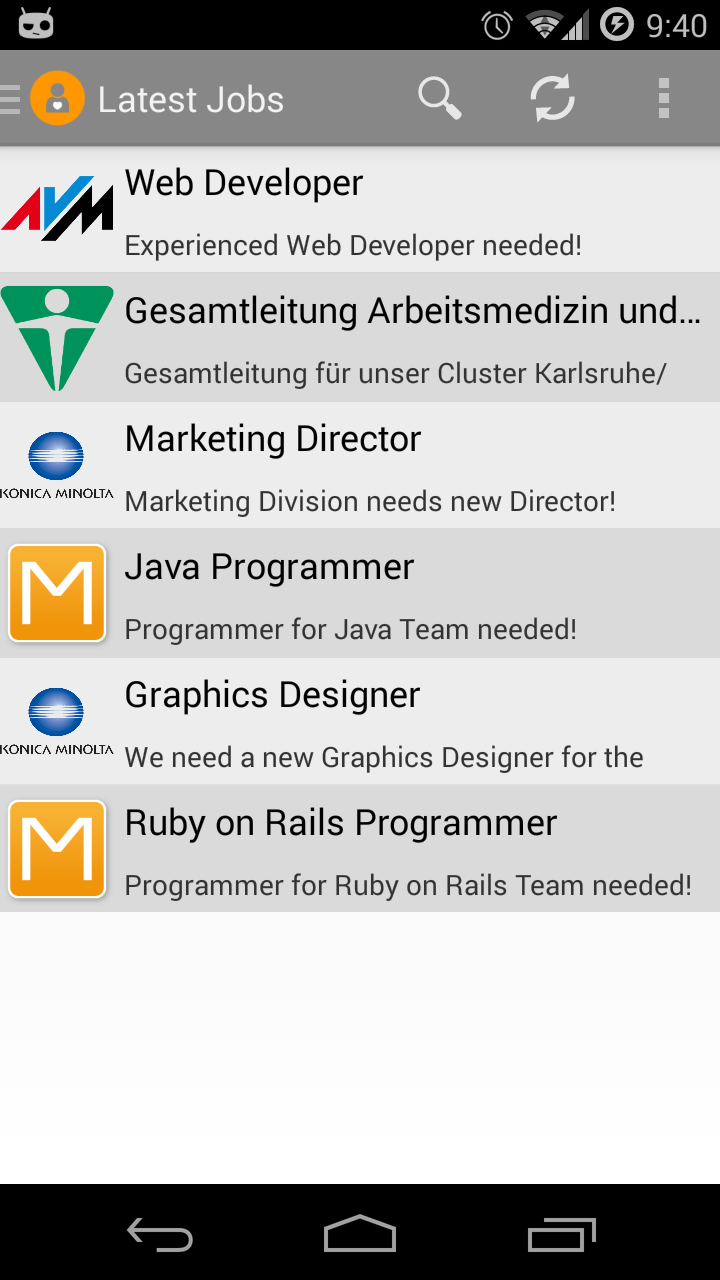
\includegraphics[width=.3\linewidth]{gfx/and/main}} \\
        \caption[Publications View]{Publications View}
\end{figure}

If you click on the menu icon, you'll see a second list slide form the left side of the screen. In here you'll find the entries for the navigation menu. You can go to the companies view, or return to the home view. You'll also notice a difference between iOS and Android. iOS has an extra entry on the menu for the search view, while Android can preform the search from the top bar.

\begin{figure}[H]
        \myfloatalign
        \subfloat[iOS]
        {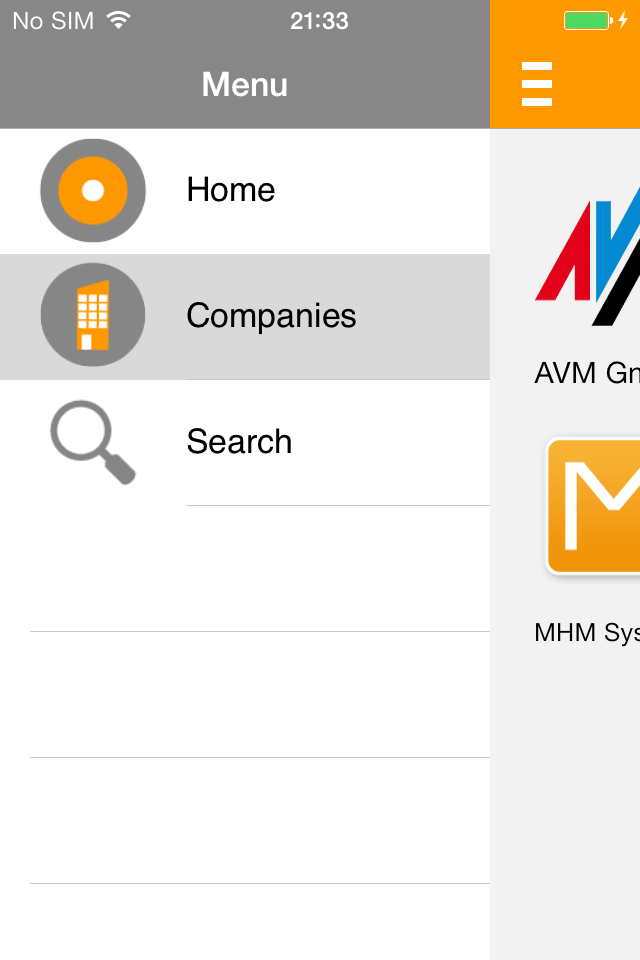
\includegraphics[width=.3\linewidth]{gfx/ios/menu}} \quad
        \subfloat[Android]
        {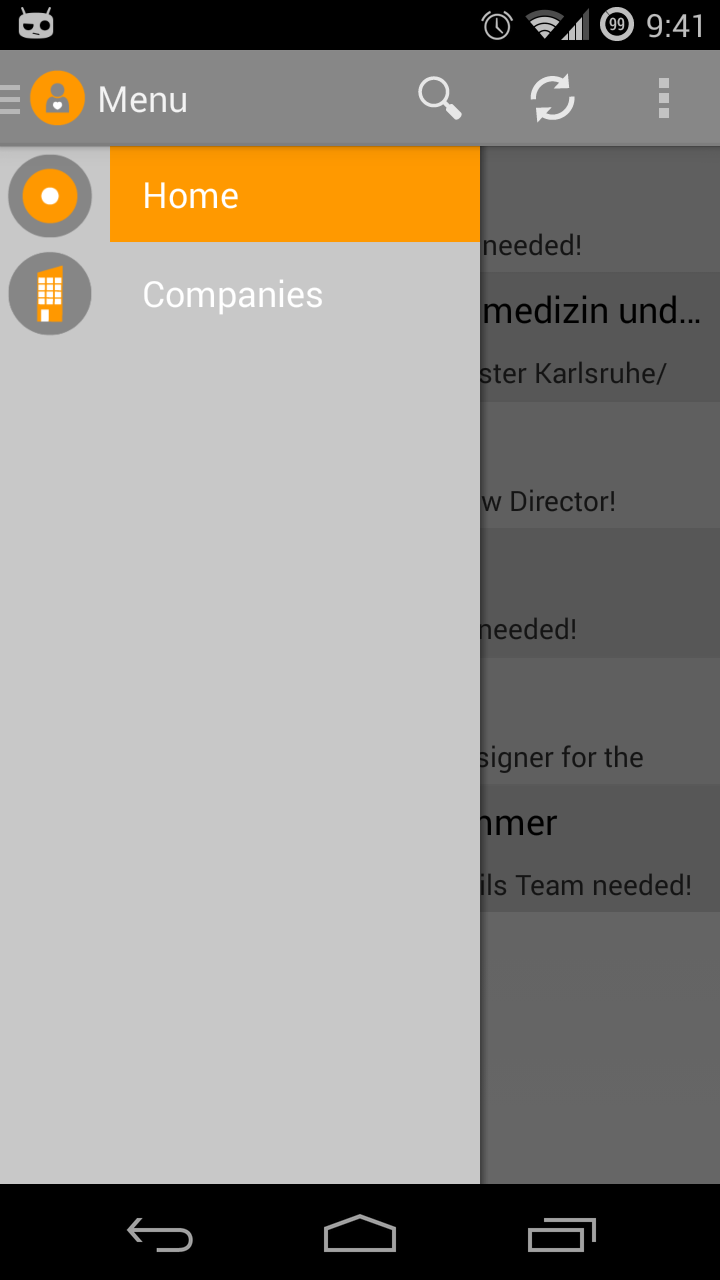
\includegraphics[width=.3\linewidth]{gfx/and/menu}} \\
        \caption[Menu]{Menu}
\end{figure}
\newpage

From there we can go the the companies view and see a grid with the available companies.

\begin{figure}[H]
        \myfloatalign
        \subfloat[iOS]
        {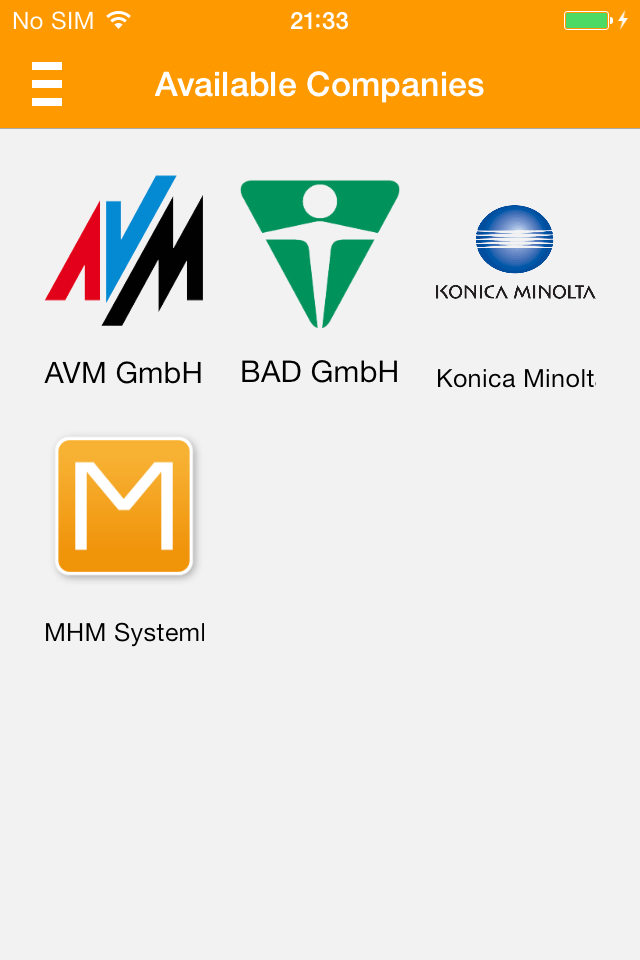
\includegraphics[width=.3\linewidth]{gfx/ios/companies}} \quad
        \subfloat[Android]
        {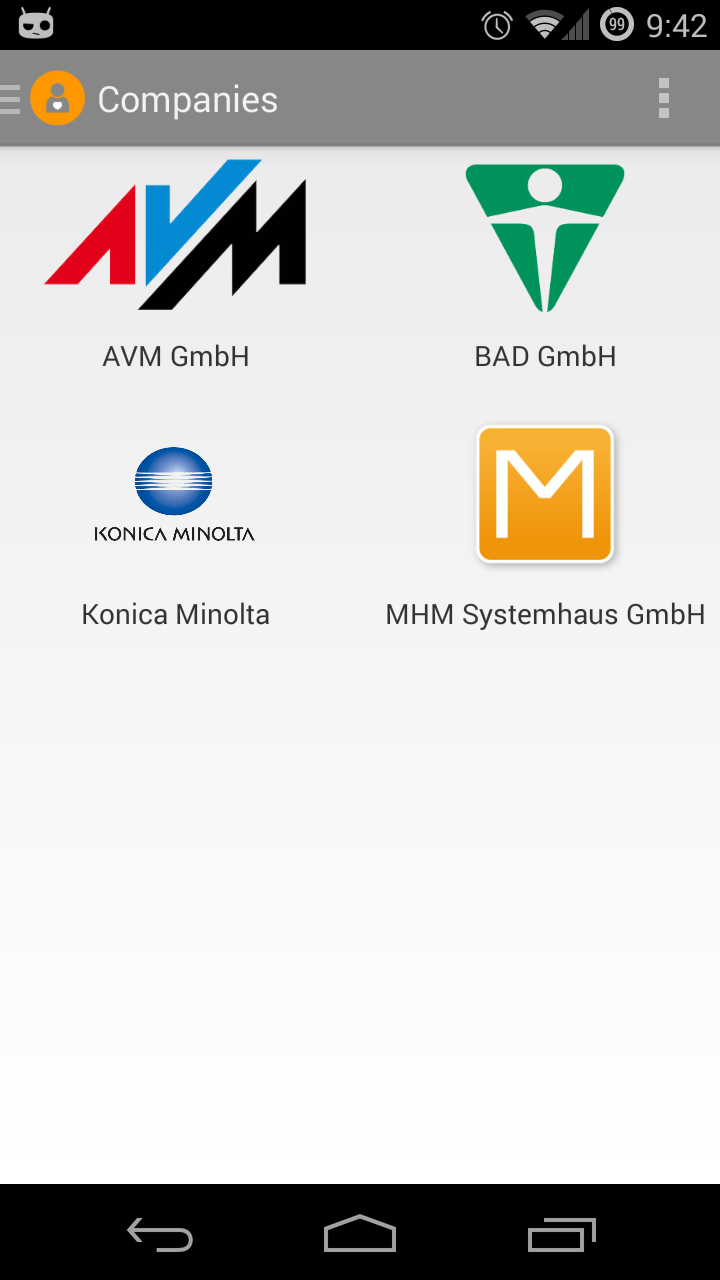
\includegraphics[width=.3\linewidth]{gfx/and/companies}} \\
        \caption[Companies View]{Companies View}
\end{figure}

Let's continue moving forward and click on a company. We will be greeted by a very similar view as the home view, but with filtered publications.

\begin{figure}[H]
        \myfloatalign
        \subfloat[iOS]
        {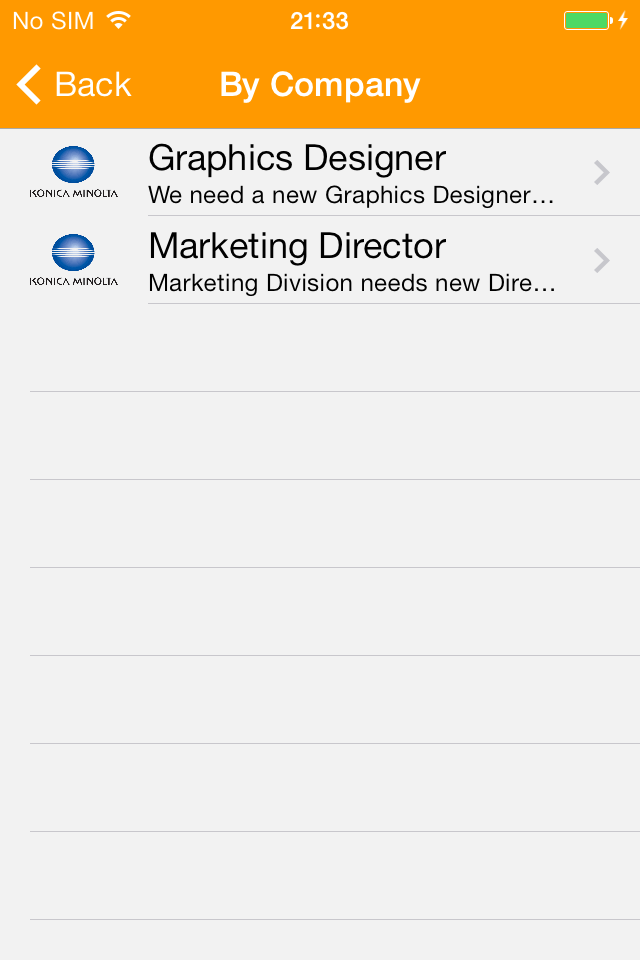
\includegraphics[width=.3\linewidth]{gfx/ios/filtered}} \quad
        \subfloat[Android]
        {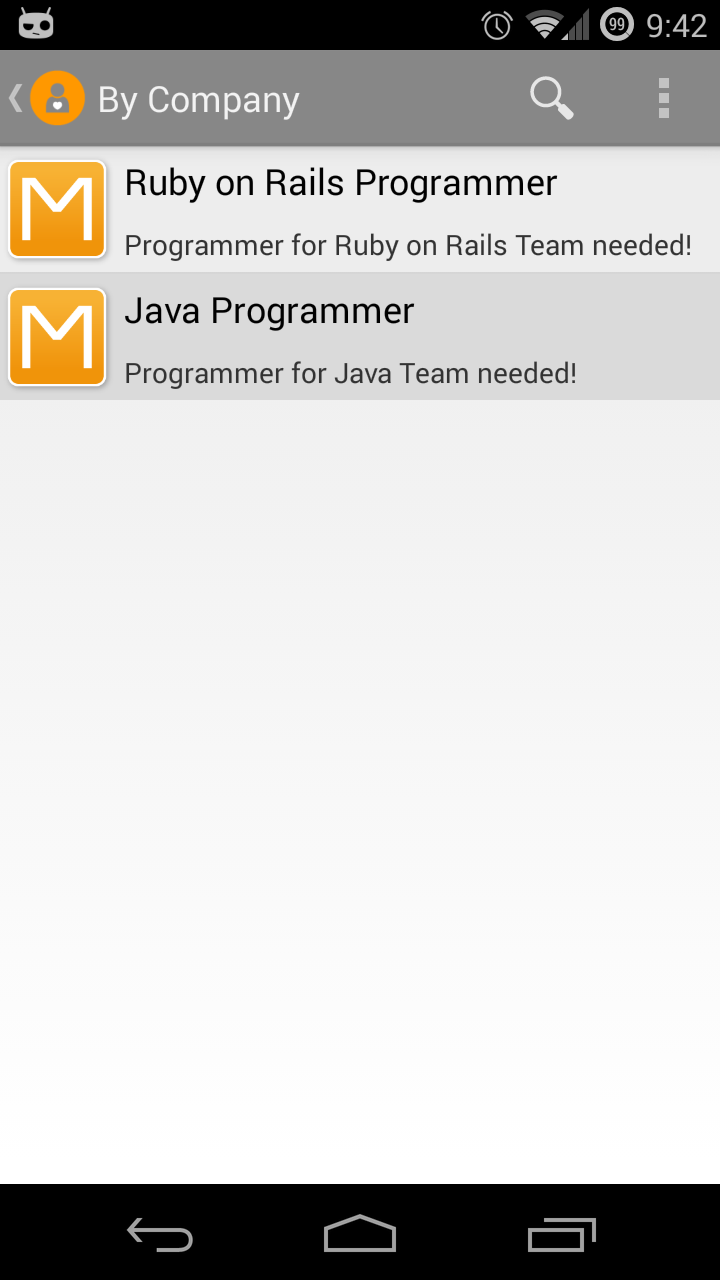
\includegraphics[width=.3\linewidth]{gfx/and/filtered}} \\
        \caption[Filtered View]{Filtered View}
\end{figure}

Let's now click on a Publication to see more details about it. A new view appears. This new view disables the menu icon and replaces it with a back button for navigation.

\begin{figure}[H]
        \myfloatalign
        \subfloat[iOS]
        {
\includegraphics[width=.3\linewidth]{gfx/ios/job}} \quad
        \subfloat[Android]
        {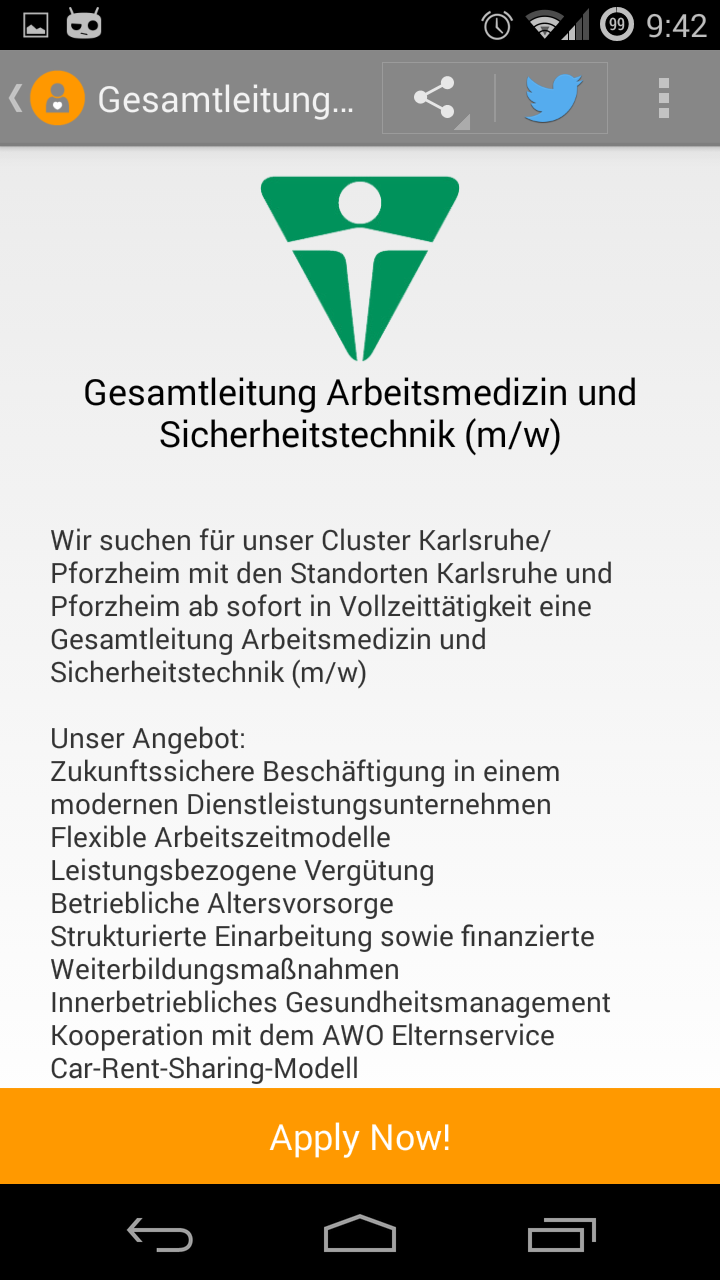
\includegraphics[width=.3\linewidth]{gfx/and/job}} \\
        \caption[Filtered View]{Filtered View}
\end{figure}

Inside this view you'll also see an "Apply Now!" button (iOS users need to scroll to the bottom). If you click this button you will be taken to a web view, that let's you directly apply to this vacancy via the responsive web interface of the \textit{MHM eRecruiting Application}.

\begin{figure}[H]
        \myfloatalign
        \subfloat[iOS]
        {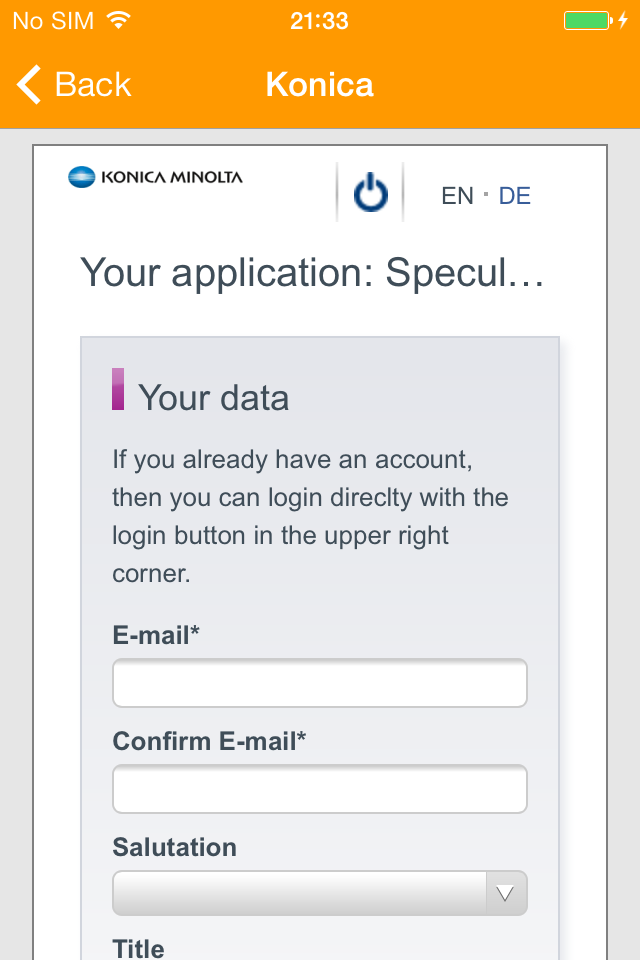
\includegraphics[width=.3\linewidth]{gfx/ios/web}} \quad
        \subfloat[Android]
        {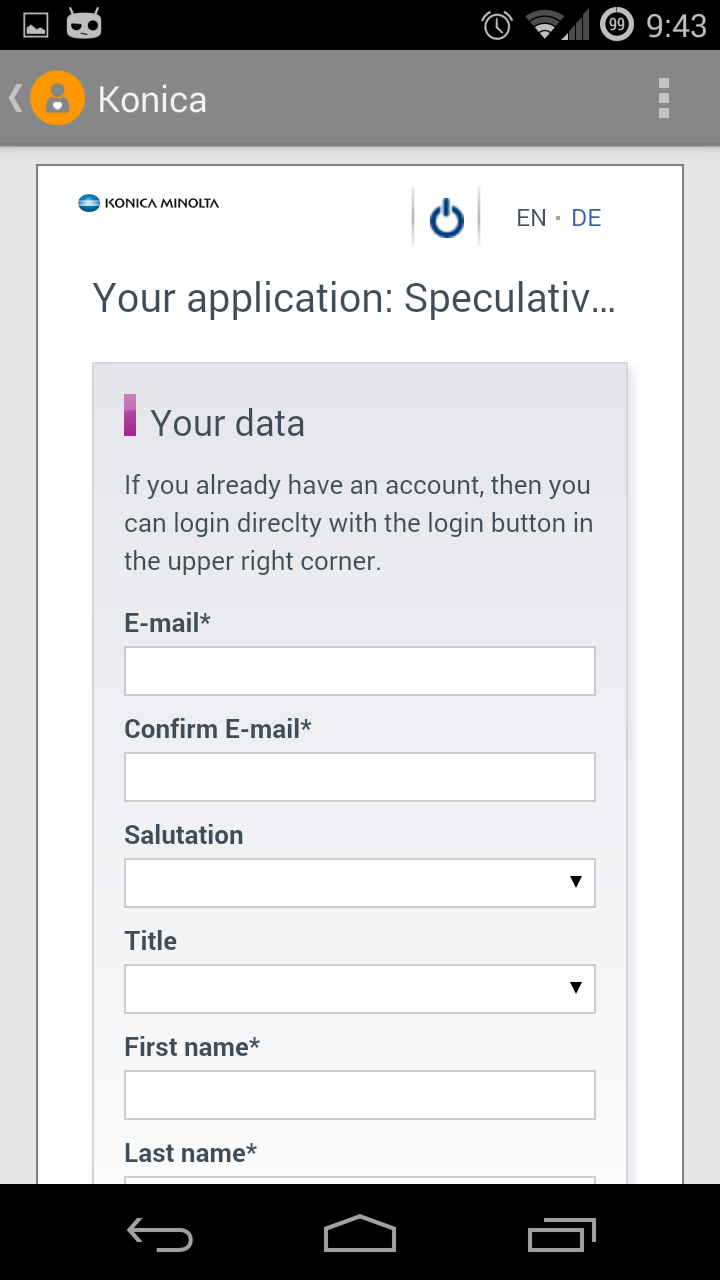
\includegraphics[width=.3\linewidth]{gfx/and/web}} \\
        \caption[Web View]{Web View}
\end{figure}

Let's go back to the navigation menu and click on search, or in Android's case, click the search icon in the top bar and type a search query. Once you start typing you'll notice the next difference. Android displays past searches as suggestions right underneath the search field. This feature was not implemented under iOS due to time constraints. Another big difference is that iOS can immediately begin to show results, while for Android to show the results, you need to click on 'Done'. This behavior is possible on Android, but requires a more complex implementation.

\begin{figure}[H]
        \myfloatalign
        \subfloat[iOS]
        {
\includegraphics[width=.3\linewidth]{gfx/ios/search}} \quad
        \subfloat[Android]
        {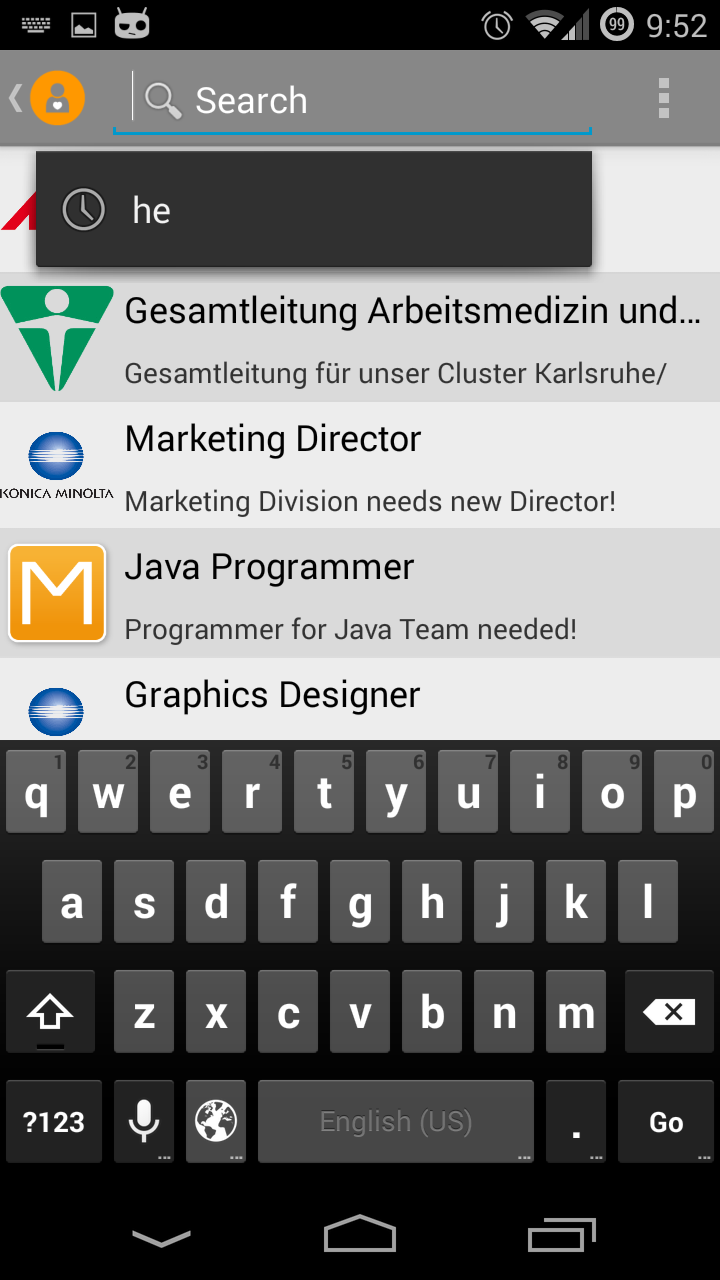
\includegraphics[width=.3\linewidth]{gfx/and/search}} \\
        \caption[Search View]{Search View}
\end{figure}

We can also refresh the main view, to see if new Publications have been made available. For this we need to go back to "Home" and, under iOS, pull the table down and release it, or, under Android, click on the refresh button.

\begin{figure}[H]
        \myfloatalign
        \subfloat[iOS]
        {
\includegraphics[width=.3\linewidth]{gfx/ios/refresh}} \quad
        \subfloat[Android]
        {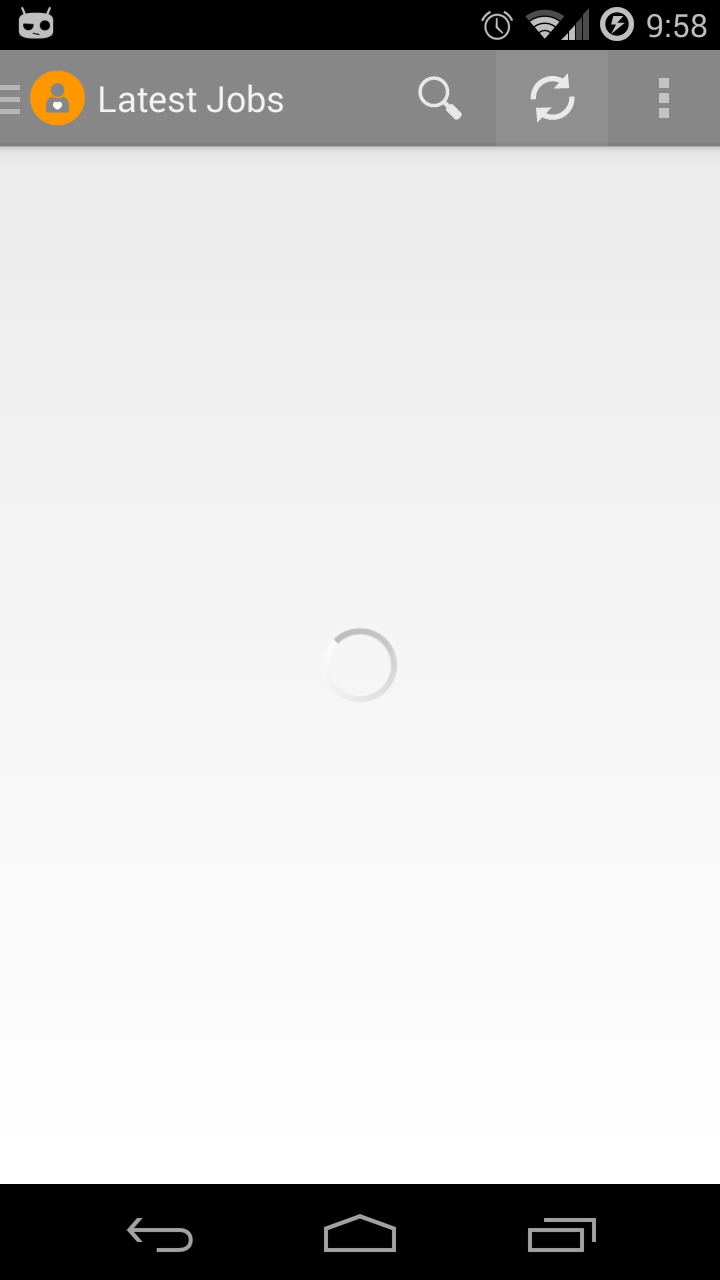
\includegraphics[width=.3\linewidth]{gfx/and/refresh}} \\
        \caption[Refreshing]{Refreshing}
\end{figure}
\newpage

There are also the possibility to display error messages, in case something goes wrong during the asynchronous connections.

\begin{figure}[H]
        \myfloatalign
        \subfloat[iOS]
        {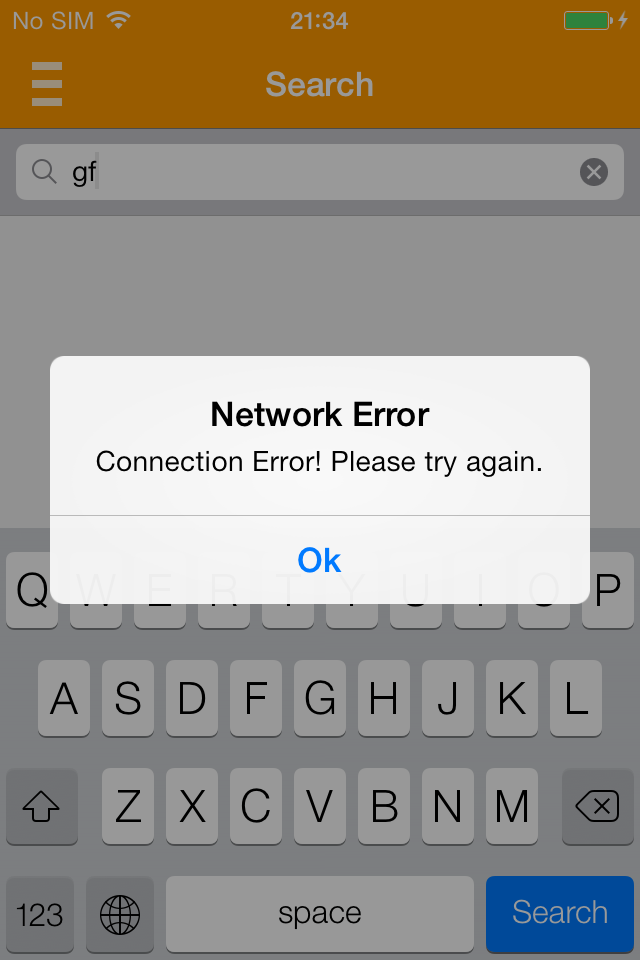
\includegraphics[width=.3\linewidth]{gfx/ios/error}} \quad
        \subfloat[Android]
        {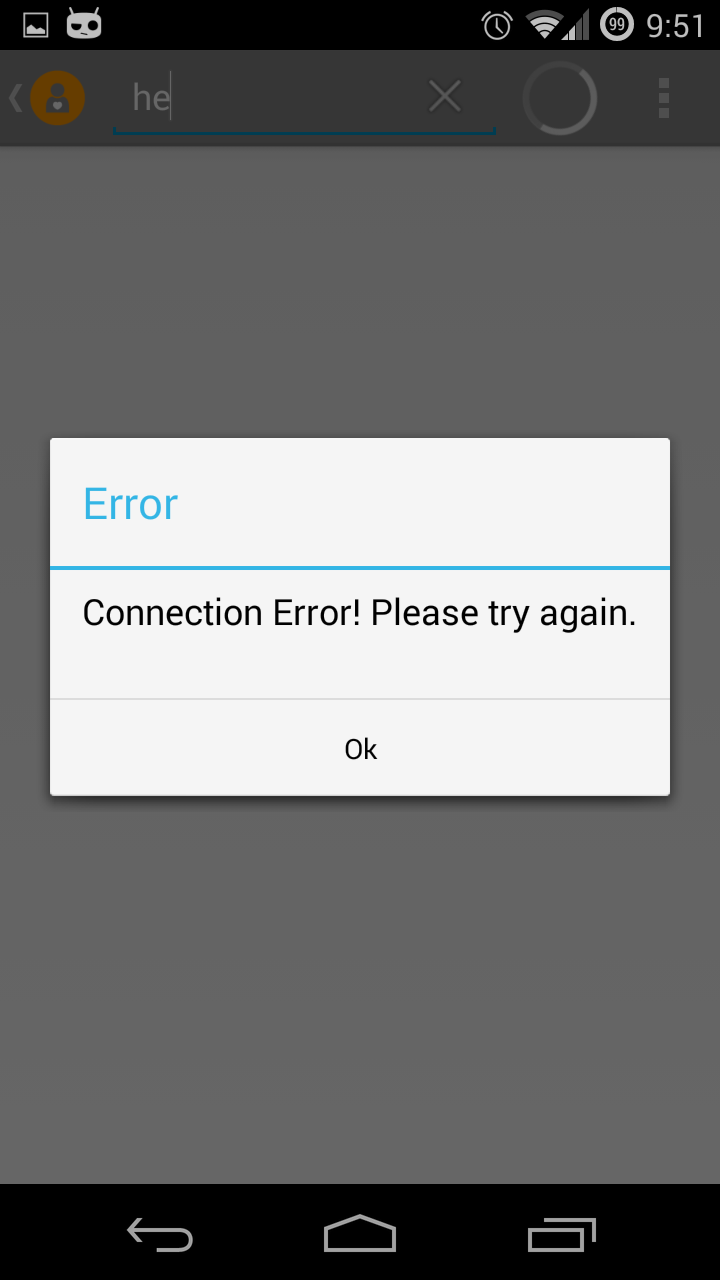
\includegraphics[width=.3\linewidth]{gfx/and/error}} \\
        \caption[Error Messages]{Error Messages}
\end{figure}

Another feature that should be displayed here is the ability to receive push notifications. Even though this functionality is implemented inside both applications, there is no server to actually send the notifications yet. This feature will be added to server soon and will be available once the application goes into production.





 

 
%************************************************
\chapter{Placeholder}\label{ch:introduction}
%************************************************
%\include{multiToC} % <--- just debug stuff, ignore for your documents
% ********************************************************************
% Backmatter
%*******************************************************
\appendix
\cleardoublepage
%\part{Appendix}
%********************************************************************
% Appendix
%*******************************************************
% If problems with the headers: get headings in appendix etc. right
%\markboth{\spacedlowsmallcaps{Appendix}}{\spacedlowsmallcaps{Appendix}}
\chapter{Appendix Test}
Lorem ipsum at nusquam appellantur his, ut eos erant homero
concludaturque. Albucius appellantur deterruisset id eam, vivendum
partiendo dissentiet ei ius. Vis melius facilisis ea, sea id convenire
referrentur, takimata adolescens ex duo. Ei harum argumentum per. Eam
vidit exerci appetere ad, ut vel zzril intellegam interpretaris.

Errem omnium ea per, pro congue populo ornatus cu, ex qui dicant
nemore melius. No pri diam iriure euismod. Graecis eleifend
appellantur quo id. Id corpora inimicus nam, facer nonummy ne pro,
kasd repudiandae ei mei. Mea menandri mediocrem dissentiet cu, ex
nominati imperdiet nec, sea odio duis vocent ei. Tempor everti
appareat cu ius, ridens audiam an qui, aliquid admodum conceptam ne
qui. Vis ea melius nostrum, mel alienum euripidis eu.

\section{Appendix Section Test}
Ei choro aeterno antiopam mea, labitur bonorum pri no. His no decore
nemore graecis. In eos meis nominavi, liber soluta vim cu. Sea commune
suavitate interpretaris eu, vix eu libris efficiantur.

\graffito{More dummy text.}
Nulla fastidii ea ius, exerci suscipit instructior te nam, in ullum
postulant quo. Congue quaestio philosophia his at, sea odio autem
vulputate ex. Cu usu mucius iisque voluptua. Sit maiorum propriae at,
ea cum primis intellegat. Hinc cotidieque reprehendunt eu nec. Autem
timeam deleniti usu id, in nec nibh altera.

\section{Another Appendix Section Test}
Equidem detraxit cu nam, vix eu delenit periculis. Eos ut vero
constituto, no vidit propriae complectitur sea. Diceret nonummy in
has, no qui eligendi recteque consetetur. Mel eu dictas suscipiantur,
et sed placerat oporteat. At ipsum electram mei, ad aeque atomorum
mea.

\begin{table}
    \myfloatalign
  \begin{tabularx}{\textwidth}{Xll} \toprule
    \tableheadline{labitur bonorum pri no} & \tableheadline{que vista}
    & \tableheadline{human} \\ \midrule
    fastidii ea ius & germano &  demonstratea \\
    suscipit instructior & titulo & personas \\
    %postulant quo & westeuropee & sanctificatec \\
    \midrule
    quaestio philosophia & facto & demonstrated \\
    %autem vulputate ex & parola & romanic \\
    %usu mucius iisque & studio & sanctificatef \\
    \bottomrule
  \end{tabularx}
  \caption[Autem usu id]{Autem usu id.}
  \label{tab:moreexample}
\end{table}

Ei solet nemore consectetuer nam. Ad eam porro impetus, te choro omnes
evertitur mel. Molestie conclusionemque vel at, no qui omittam
expetenda efficiendi. Eu quo nobis offendit, verterem scriptorem ne
vix.

  
\begin{lstlisting}[float,caption=A floating example]
for i:=maxint to 0 do
begin
{ do nothing }
end;
\end{lstlisting}
%********************************************************************
% Other Stuff in the Back
%*******************************************************
\cleardoublepage%********************************************************************
% Bibliography
%*******************************************************
% work-around to have small caps also here in the headline
\manualmark
\markboth{\spacedlowsmallcaps{\bibname}}{\spacedlowsmallcaps{\bibname}} % work-around to have small caps also
%\phantomsection 
\refstepcounter{dummy}
\addtocontents{toc}{\protect\vspace{\beforebibskip}} % to have the bib a bit from the rest in the toc
\addcontentsline{toc}{chapter}{\tocEntry{\bibname}}
\bibliographystyle{plainnat}
\label{app:bibliography} 
\bibliography{Bibliography}
\cleardoublepage\pagestyle{empty}

\hfill

\vfill


\pdfbookmark[0]{Colophon}{colophon}
\section*{Colophon}
This document was typeset using the typographical look-and-feel \texttt{classicthesis} developed by Andr\'e Miede. 
The style was inspired by Robert Bringhurst's seminal book on typography ``\emph{The Elements of Typographic Style}''. 
\texttt{classicthesis} is available for both \LaTeX\ and \mLyX: 
\begin{center}
\url{http://code.google.com/p/classicthesis/}
\end{center}
Happy users of \texttt{classicthesis} usually send a real postcard to the author, a collection of postcards received so far is featured here: 
\begin{center}
\url{http://postcards.miede.de/}
\end{center}
 
\bigskip

\noindent\finalVersionString

%Hermann Zapf's \emph{Palatino} and \emph{Euler} type faces (Type~1 PostScript fonts \emph{URW
%Palladio L} and \emph{FPL}) are used. The ``typewriter'' text is typeset in \emph{Bera Mono}, 
%originally developed by Bitstream, Inc. as ``Bitstream Vera''. (Type~1 PostScript fonts were made 
%available by Malte Rosenau and
%Ulrich Dirr.)

%\paragraph{note:} The custom size of the textblock was calculated
%using the directions given by Mr. Bringhurst (pages 26--29 and
%175/176). 10~pt Palatino needs  133.21~pt for the string
%``abcdefghijklmnopqrstuvwxyz''. This yields a good line length between
%24--26~pc (288--312~pt). Using a ``\emph{double square textblock}''
%with a 1:2 ratio this results in a textblock of 312:624~pt (which
%includes the headline in this design). A good alternative would be the
%``\emph{golden section textblock}'' with a ratio of 1:1.62, here
%312:505.44~pt. For comparison, \texttt{DIV9} of the \texttt{typearea}
%package results in a line length of 389~pt (32.4~pc), which is by far
%too long. However, this information will only be of interest for
%hardcore pseudo-typographers like me.%
%
%To make your own calculations, use the following commands and look up
%the corresponding lengths in the book:
%\begin{verbatim}
%    \settowidth{\abcd}{abcdefghijklmnopqrstuvwxyz}
%    \the\abcd\ % prints the value of the length
%\end{verbatim}
%Please see the file \texttt{classicthesis.sty} for some precalculated 
%values for Palatino and Minion.
%
%    \settowidth{\abcd}{abcdefghijklmnopqrstuvwxyz}
%    \the\abcd\ % prints the value of the length





% ********************************************************************
% Game Over: Restore, Restart, or Quit?
%*******************************************************
\end{document}
% ********************************************************************
